\chapter{Zbiór testowy obrazów skalnych}
Głównym celem niniejszej pracy był dobór metod selekcji punktów charakterystycznych pod kątem rozpoznawania obrazów skalnych. W tym celu opracowano autorski zbiór zestawów testowych służący ocenie pracy algorytmów. Zdjęcie powstały w lecie 2012 roku, w rejonie Gór Sokolich na Dolnym Śląsku. Zbiór składa się z 6 zestawów odpowiadających transformacjom takim jaki:
\begin{itemize}
\item rotacja
\item zmiana położenia obserwatora
\item zmiana skali
\end{itemize}
\FloatBarrier
\newpage
\section{Rotacja}
Rotacja jest reprezentowana przez 3 zbiory. Zbiory te różnią się między sobą skala wykadrowania zdjęcia i stopniem oświetlenia. Zostały wykonane w rejonie formacji Sukiennic, Krzywej Turni i Małego Sokolika.
\FloatBarrier
\subsection{R1}
Transformacja: Rotacja\\
Rejon: Sukiennice\\
Powiększenie: Duże\\
Oświetlenie: Duże\\
Rozdzielczość: $768 \times 768$\\
\begin{figure}[!htbp]
\begin{center}
\subfigure[R1 1]{
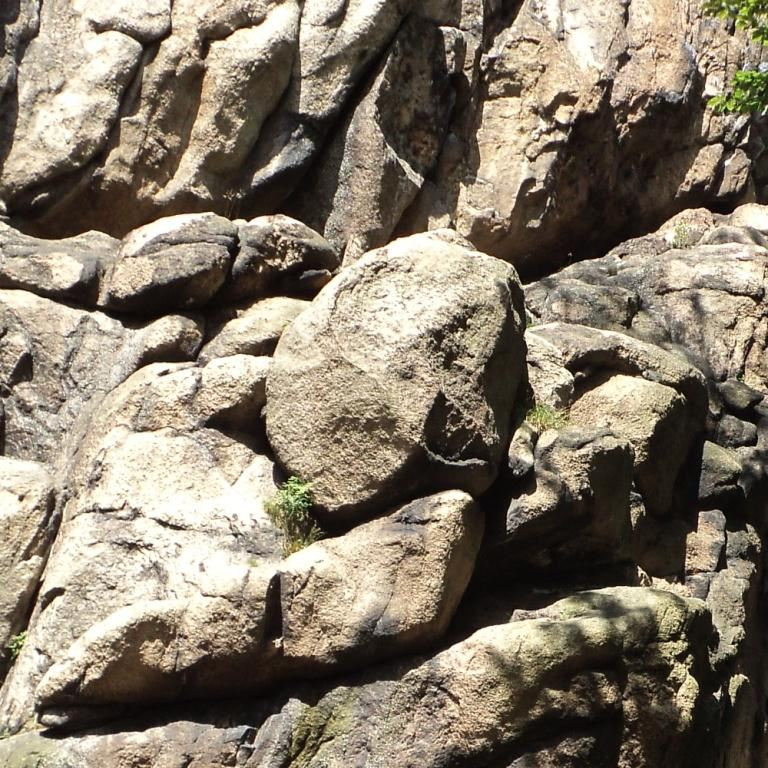
\includegraphics[width=5cm]{pict/slowik/r1/img1.jpg}
}
\subfigure[R1 2]{
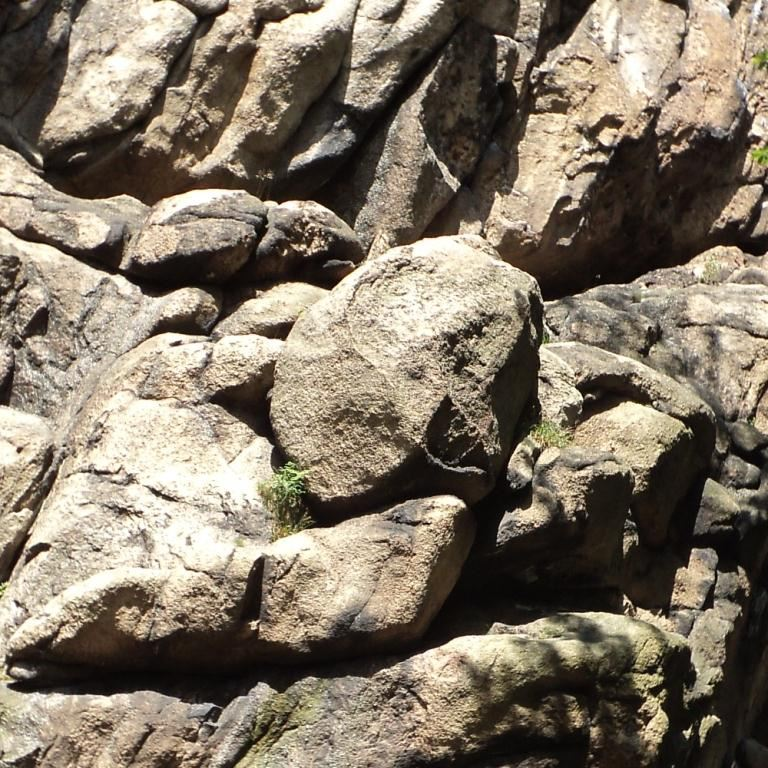
\includegraphics[width=5cm]{pict/slowik/r1/img2.jpg}
}
\subfigure[R1 3]{
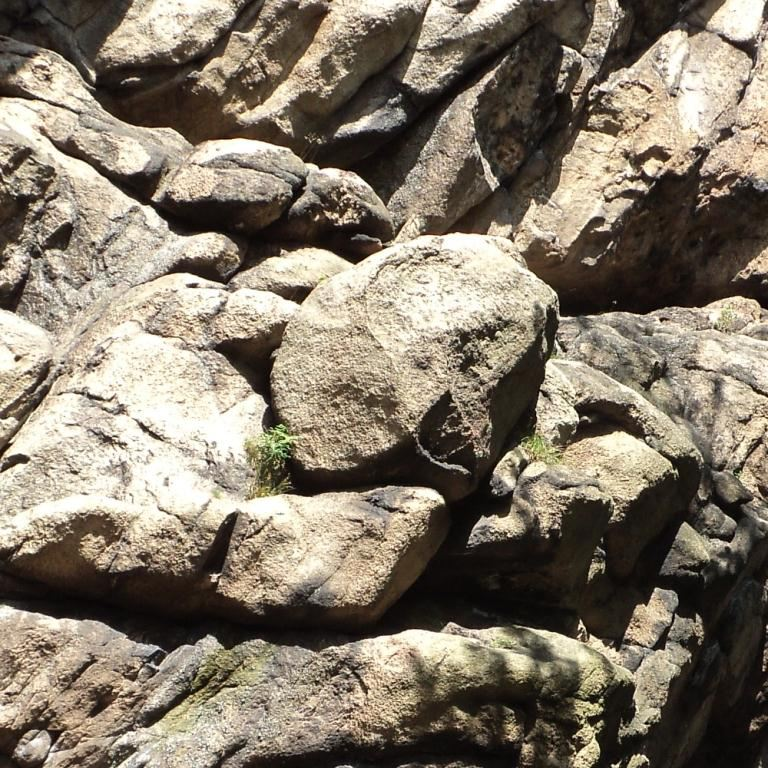
\includegraphics[width=5cm]{pict/slowik/r1/img3.jpg}
}
\subfigure[R1 4]{
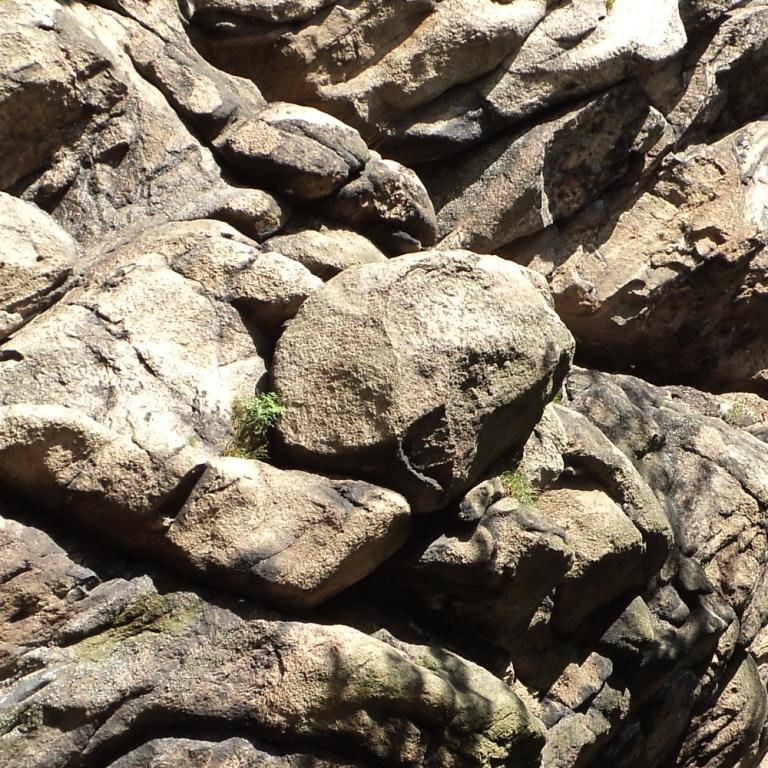
\includegraphics[width=5cm]{pict/slowik/r1/img4.jpg}
}
\subfigure[R1 5]{
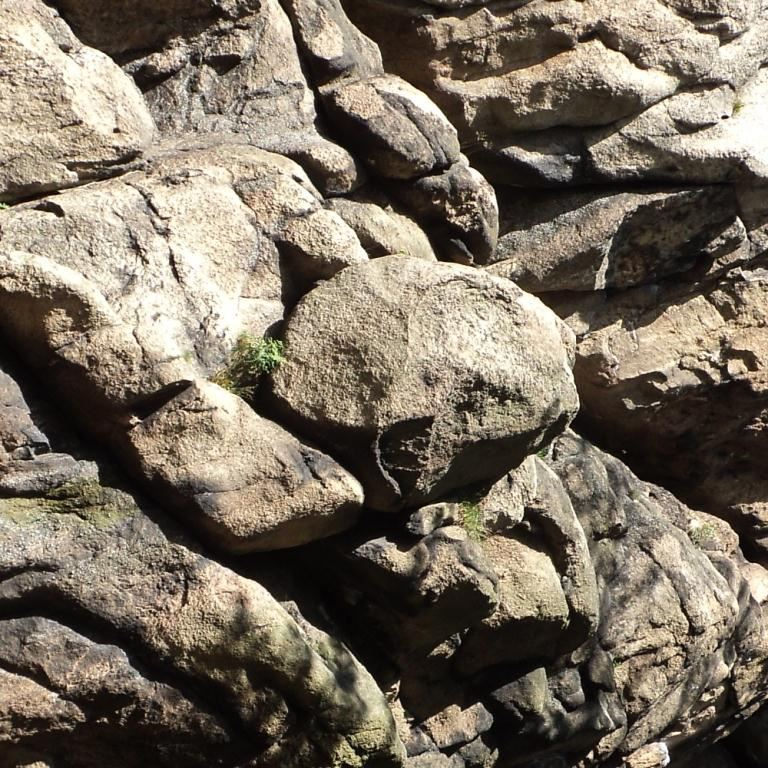
\includegraphics[width=5cm]{pict/slowik/r1/img5.jpg}
}
\subfigure[R1 6]{
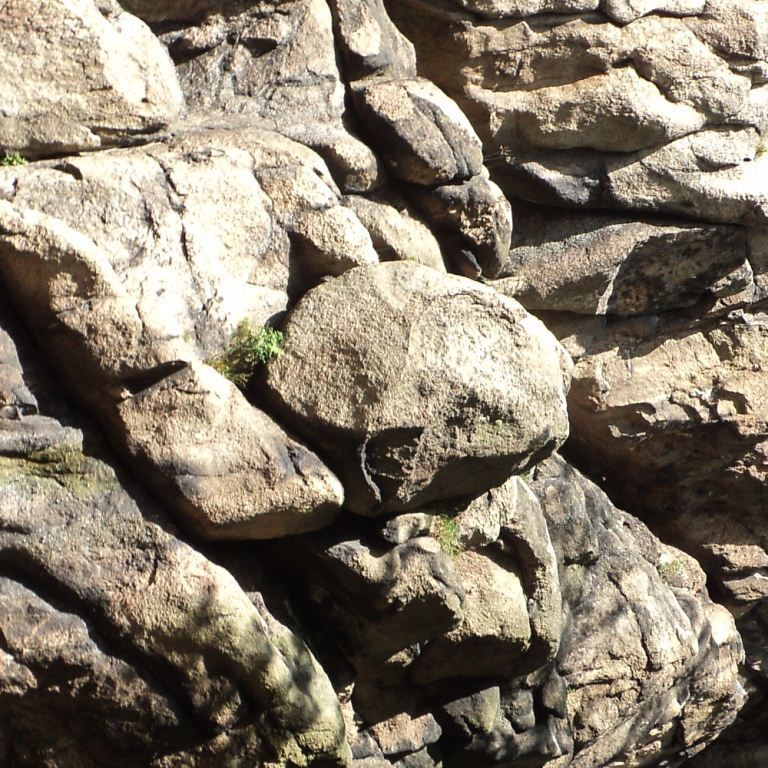
\includegraphics[width=5cm]{pict/slowik/r1/img6.jpg}
}
\caption{R1 - zbiór obrazów testowych}
\label{fig:r1_set}
\end{center}
\end{figure}

% Table generated by Excel2LaTeX from sheet 'm.r1 F'
\begin{table}[htbp]
  \centering
  \caption{R1 - ilość wyszukanych cech}
    \begin{tabular}{|c|r|r|r|r|r|}\hline
    
    obraz & \textbf{ORB} & \textbf{SIFT} & \textbf{SURF} & \textbf{STAR} & \textbf{FAST} \\\hline
   
    1 & 500 & 1795 & 8212 & 1545 & 24151 \\
    2 & 500 & 1762 & 8059 & 1555 & 23688 \\
    3 & 500 & 1729 & 8560 & 1566 & 25404 \\
    4 & 500 & 1749 & 8951 & 1601 & 25762 \\
    5 & 500 & 1678 & 8952 & 1591 & 26614 \\
    6 & 500 & 1827 & 8240 & 1596 & 23200 \\\hline
    \textbf{średnia} & \textbf{500} & \textbf{1757} & \textbf{8496} & \textbf{1576} & \textbf{24803} \\
   \hline
    \end{tabular}%
  \label{tab:r1_f1}%
\end{table}%


\begin{figure}[!htbp]
\centering
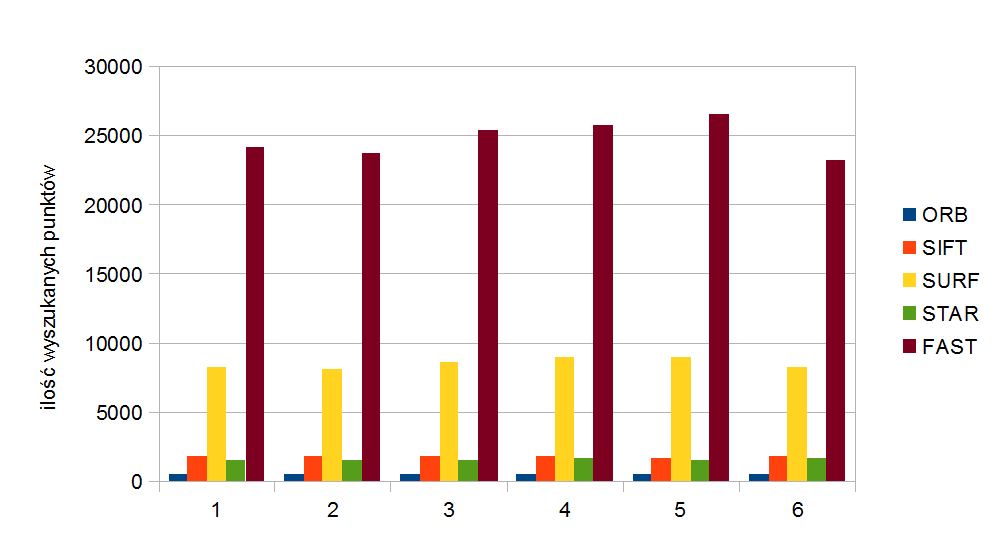
\includegraphics[width=0.8\textwidth]{pict/slowik/r1/f1.png}
\caption{R1 - ilość wyszukanych cech}
\label{fig:r1_f1}
\end{figure}


% Table generated by Excel2LaTeX from sheet 'm.r1 F'
\begin{table}[htbp]
  \centering
  \caption{R1 - czas lokalizowania pojedynczego punktu charakterystycznego}
    \begin{tabular}{|c|c|c|c|c|c|}
    \hline
    obraz & \textbf{ORB} & \textbf{SIFT} & \textbf{SURF} & \textbf{STAR} & \textbf{FAST} \\
    \hline
    -  & [ms] & [ms] & [ms] & [ms] & [ms] \\\hline
    1 & 0,152 & 0,096 & 0,166 & 0,039 & 0,001 \\
    2 & 0,150 & 0,099 & 0,166 & 0,039 & 0,001 \\
    3 & 0,154 & 0,099 & 0,165 & 0,038 & 0,001 \\
    4 & 0,158 & 0,101 & 0,164 & 0,038 & 0,001 \\
    5 & 0,158 & 0,103 & 0,163 & 0,038 & 0,001 \\
    6 & 0,152 & 0,095 & 0,166 & 0,038 & 0,001 \\\hline
    \textbf{średnia} & \textbf{0,154} & \textbf{0,099} & \textbf{0,165} & \textbf{0,038} & \textbf{0,001} \\
    \hline
    \end{tabular}%
  \label{tab:r1_f2}%
\end{table}%


\begin{figure}[htbp]
\centering
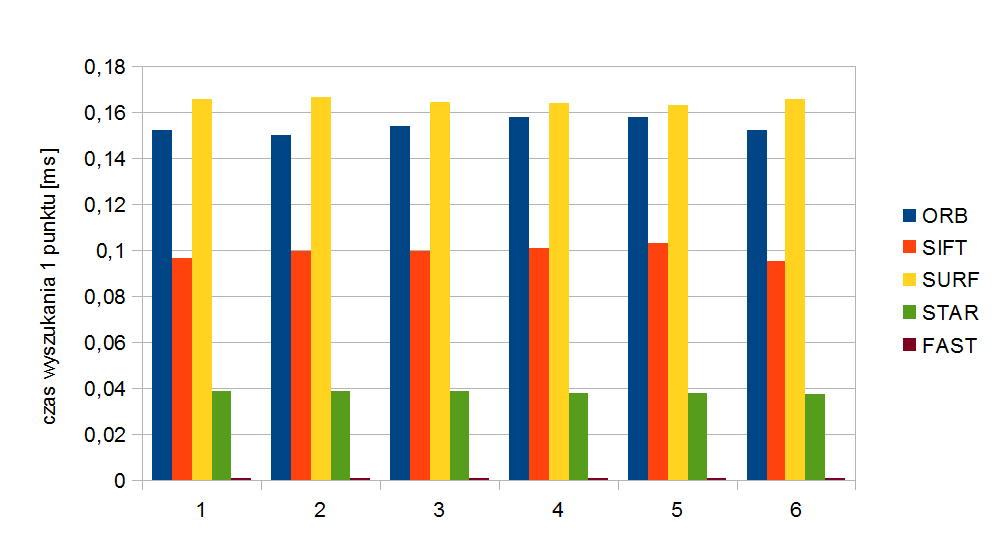
\includegraphics[width=0.8\textwidth]{pict/slowik/r1/f2.png}
\caption{R1 - czas lokalizowania pojedynczego punktu charakterystycznego}
\label{fig:r1_f2}
\end{figure}

% Table generated by Excel2LaTeX from sheet 'm.r1 F'
\begin{table}[!htbp]
  \centering
  \caption{R1 - czas generowania pojedynczego deskryptora punktu charakterystycznego}
    \begin{tabular}{|c|c|c|c|c|c|c|c|}\hline

    obraz & \textbf{ORB} & \textbf{SIFT} & \textbf{SURF} & \textbf{ST-BRIEF} & \textbf{ST-ORB} & \textbf{ST-SIFT} & \textbf{ST-SURF} \\\hline

    - & [ms] & [ms] & [ms] & [ms] & [ms] & [ms] & [ms] \\\hline
    1 & 0,078 & 0,233 & 0,187 & 0,012 & 0,012 & 1,197 & 0,098 \\
    2 & 0,080 & 0,236 & 0,186 & 0,012 & 0,013 & 1,194 & 0,098 \\
    3 & 0,082 & 0,239 & 0,187 & 0,012 & 0,012 & 1,238 & 0,099 \\
    4 & 0,078 & 0,236 & 0,185 & 0,012 & 0,012 & 1,213 & 0,097 \\
    5 & 0,078 & 0,240 & 0,185 & 0,013 & 0,013 & 1,200 & 0,099 \\
    6 & 0,080 & 0,230 & 0,190 & 0,013 & 0,013 & 1,274 & 0,098 \\\hline
    \textbf{średnia} & \textbf{0,079} & \textbf{0,236} & \textbf{0,187} & \textbf{0,012} & \textbf{0,012} & \textbf{1,219} & \textbf{0,098} \\\hline
    

    \end{tabular}%
  \label{tab:r1_f3}%
\end{table}%


\begin{figure}[!htbp]
\centering
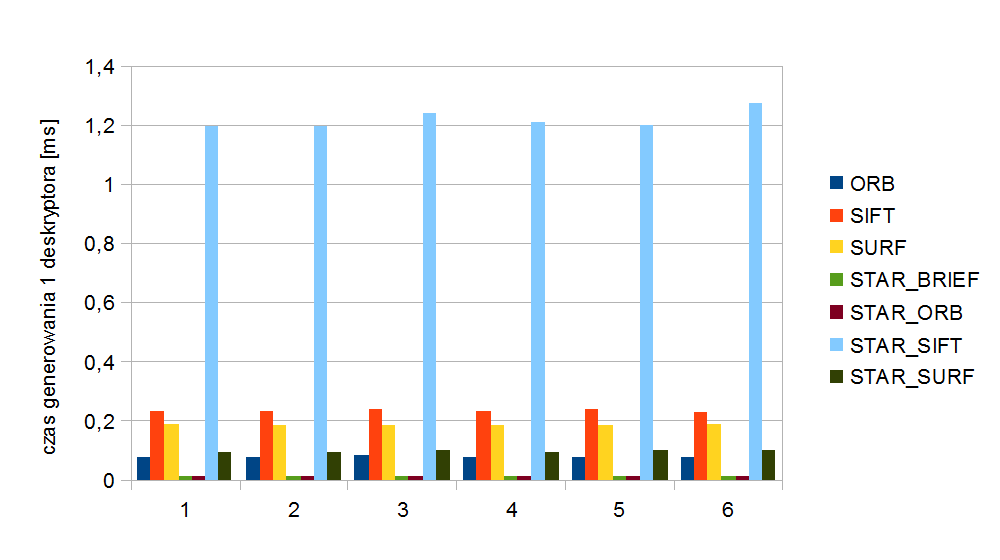
\includegraphics[width=0.8\textwidth]{pict/slowik/r1/f3.png}
\caption{R1 - czas generowania pojedynczego deskryptora punktu charakterystycznego}
\label{fig:r1_f3}
\end{figure}


% Table generated by Excel2LaTeX from sheet 'm.r1 M'
\begin{table}[htbp]
  \centering
  \caption{R1 - powtarzalność wykrywanych cech}
    \begin{tabular}{|c|c|c|c|c|c|c|c|}\hline

    obrazy & \textbf{ORB} & \textbf{SIFT} & \textbf{SURF} & \textbf{ST-BRIEF} & \textbf{ST-ORB} & \textbf{ST-SIFT} & \textbf{ST-SURF} \\\hline

    -  & [\%] & [\%] & [\%] & [\%] & [\%] & [\%] & [\%] \\\hline
    1|2 & 57 & 56 & 40 & 63 & 60 & 70 & 25 \\
    1|3 & 56 & 56 & 26 & 6 & 3 & 16 & 18 \\
    1|4 & 35 & 35 & 16 & 3 & 2 & 1 & 15 \\
    1|5 & 33 & 37 & 12 & 2 & 2 & 1 & 9 \\
    1|6 & 46 & 49 & 19 & 2 & 2 & 1 & 15 \\\hline
    \textbf{średnia} & \textbf{45} & \textbf{46} & \textbf{23} & \textbf{15} & \textbf{14} & \textbf{18} & \textbf{17} \\\hline
   
    \end{tabular}%
  \label{tab:r1_m1}%
\end{table}%


\begin{figure}[!htbp]
\centering
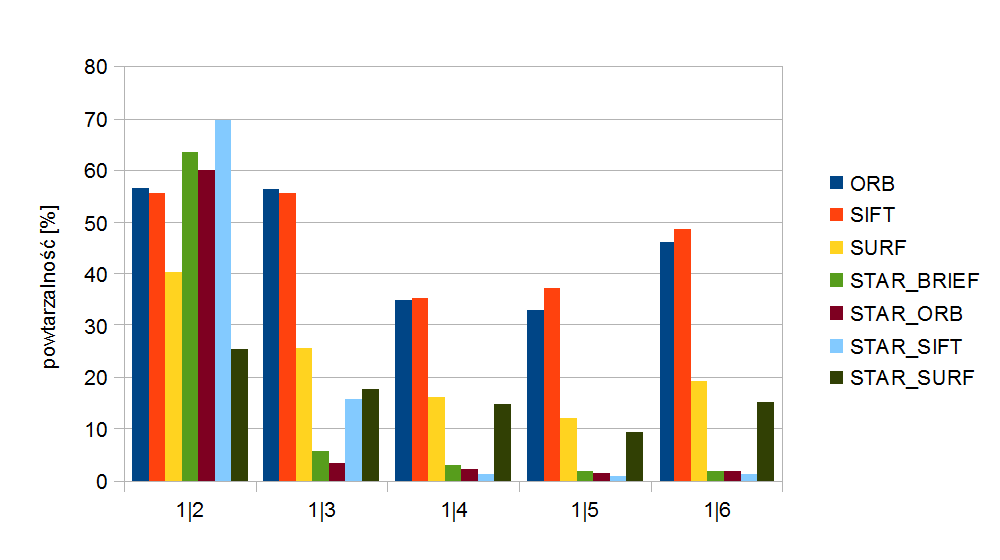
\includegraphics[width=0.8\textwidth]{pict/slowik/r1/m1.png}
\caption{R1 - powtarzalność wykrywanych cech}
\label{fig:r1_m1}
\end{figure}

% Table generated by Excel2LaTeX from sheet 'm.r1 M'
\begin{table}[htbp]
  \centering
  \caption{R1 - procent poprawnych dopasowań}
    \begin{tabular}{|c|c|c|c|c|c|c|c|}\hline
    obrazy & \textbf{ORB} & \textbf{SIFT} & \textbf{SURF} & \textbf{ST-BRIEF} & \textbf{ST-ORB} & \textbf{ST-SIFT} & \textbf{ST-SURF} \\\hline
     - & [\%] & [\%] & [\%] & [\%] & [\%] & [\%] & [\%] \\\hline
    1|2 & 76 & 85 & 68 & 70 & 68 & 80 & 68 \\
    1|3 & 84 & 94 & 52 & 62 & 39 & 80 & 65 \\
    1|4 & 60 & 60 & 46 & 8 & 9 & 14 & 63 \\
    1|5 & 49 & 64 & 34 & 9 & 8 & 16 & 38 \\
    1|6 & 55 & 55 & 38 & 10 & 8 & 24 & 43 \\\hline
    \textbf{średnia} & \textbf{65} & \textbf{71} & \textbf{47} & \textbf{32} & \textbf{26} & \textbf{43} & \textbf{55} \\\hline
    
    \end{tabular}%
  \label{tab:r1_m2}%
\end{table}%


\begin{figure}[!htbp]
\centering
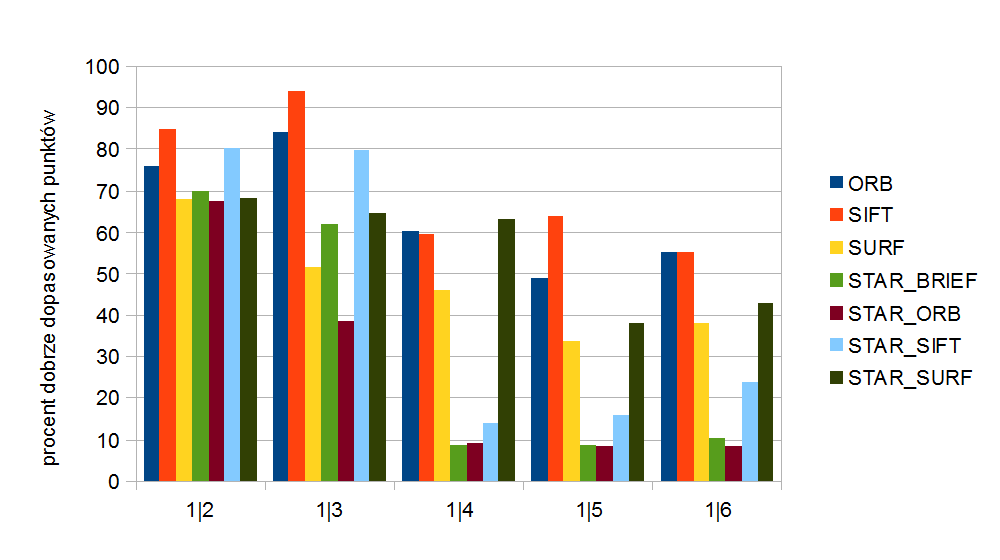
\includegraphics[width=0.8\textwidth]{pict/slowik/r1/m2.png}
\caption{R1 - procent poprawnych dopasowań}
\label{fig:r1_m2}
\end{figure}




\FloatBarrier
\newpage
\subsection{R2}
Transformacja: Rotacja\\
Rejon: Sokolik Mały\\
Powiększenie: Małe\\
Oświetlenie: Duże\\
Rozdzielczość: $768 \times 1024$\\
\begin{figure}[!htb]
\begin{center}
\subfigure[R2 1]{
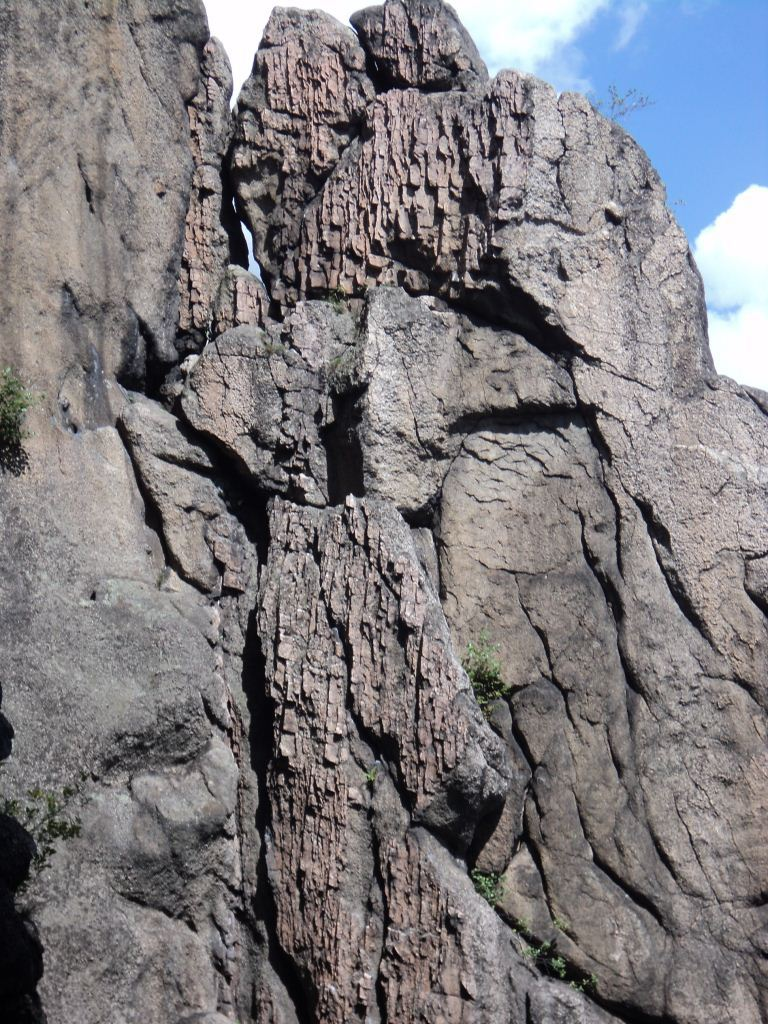
\includegraphics[width=5cm]{pict/slowik/r2/img1.jpg}
}
\subfigure[R2 2]{
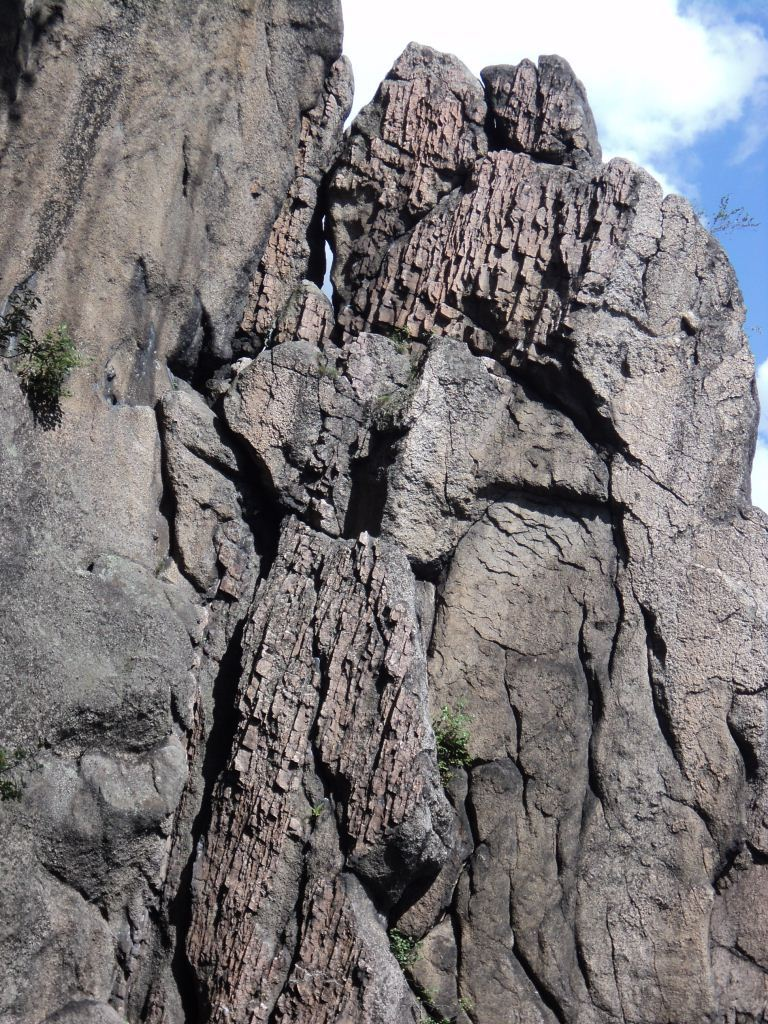
\includegraphics[width=5cm]{pict/slowik/r2/img2.jpg}
}
\subfigure[R2 3]{
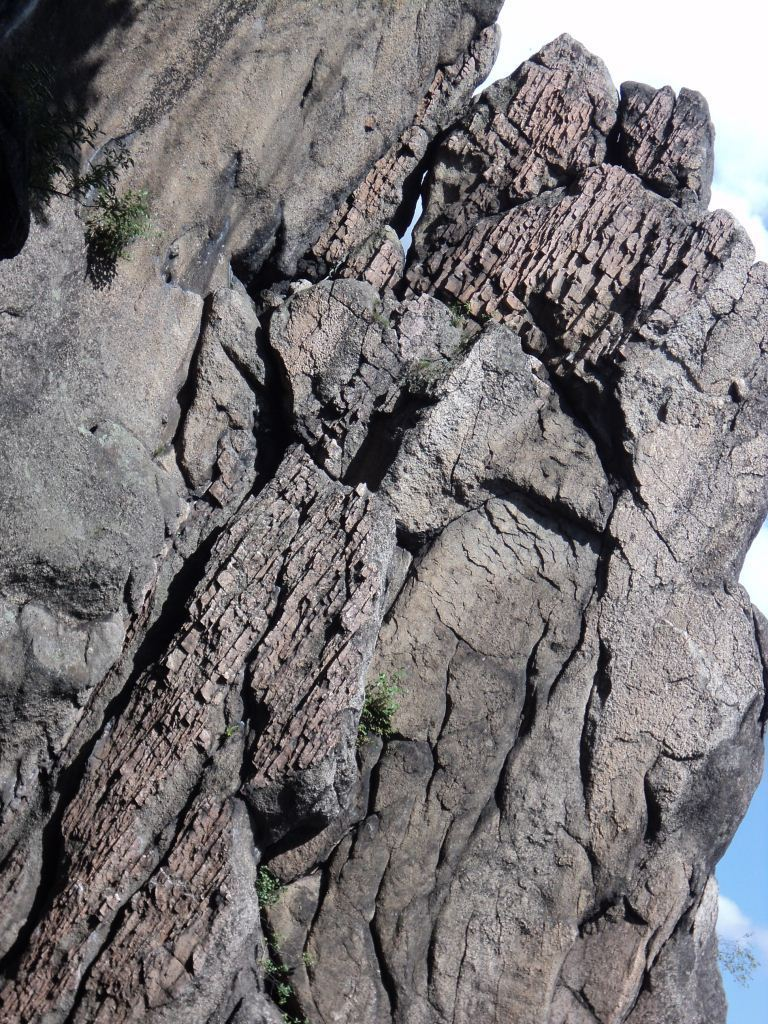
\includegraphics[width=5cm]{pict/slowik/r2/img3.jpg}
}
\subfigure[R2 4]{
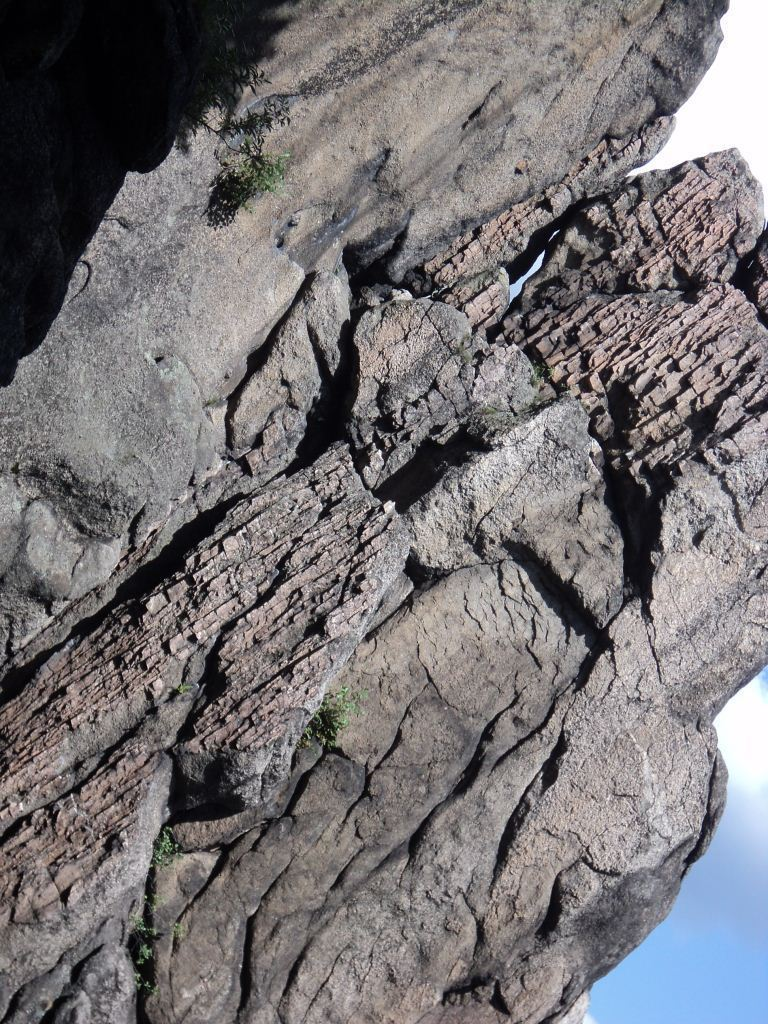
\includegraphics[width=5cm]{pict/slowik/r2/img4.jpg}
}
\subfigure[R2 5]{
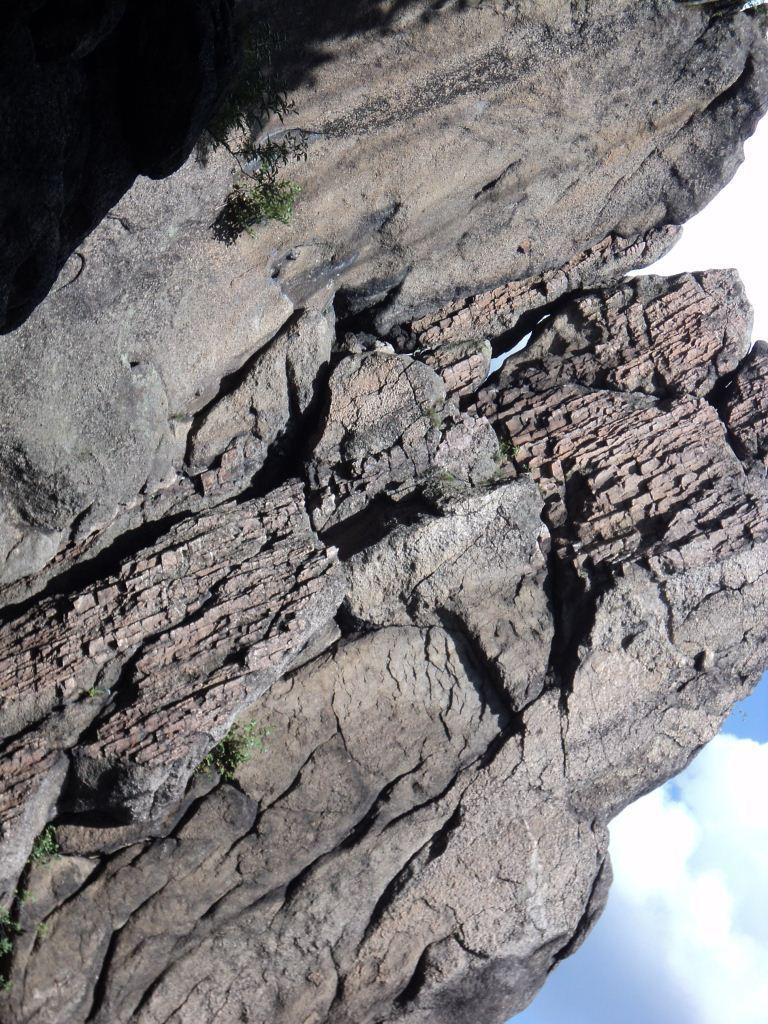
\includegraphics[width=5cm]{pict/slowik/r2/img5.jpg}
}
\subfigure[R2 6]{
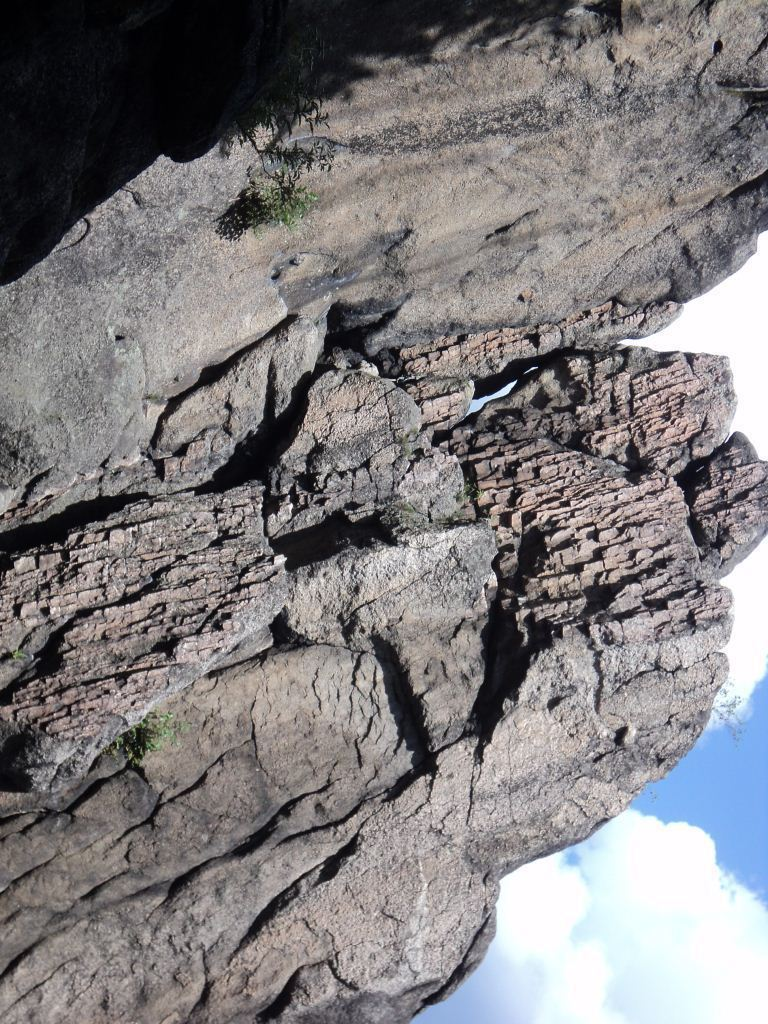
\includegraphics[width=5cm]{pict/slowik/r2/img6.jpg}
}
\caption{R2 - zbiór obrazów testowych}
\label{fig:r2_set}
\end{center}
\end{figure}



% Table generated by Excel2LaTeX from sheet 'm.r2 F'
\begin{table}[htbp]
  \centering
  \caption{ilość wyszukanych cech}
    \begin{tabular}{|c|r|r|r|r|r|}\hline
    
    obraz & \textbf{ORB} & \textbf{SIFT} & \textbf{SURF} & \textbf{STAR} & \textbf{FAST} \\\hline
    
   
    1 & 500 & 2879 & 12776 & 2834 & 39644 \\
    2 & 500 & 2844 & 14042 & 2852 & 47948 \\
    3 & 500 & 2874 & 13905 & 2912 & 48224 \\
    4 & 500 & 2741 & 13416 & 2543 & 44424 \\
    5 & 500 & 2686 & 12601 & 2343 & 40263 \\
    6 & 500 & 2600 & 12938 & 2274 & 40797 \\\hline
    \textbf{średnia} & \textbf{500} & \textbf{2771} & \textbf{13280} & \textbf{2626} & \textbf{43550} \\
    \hline
    \end{tabular}%
  \label{tab:r2_f1}%
\end{table}%


\begin{figure}
\centering
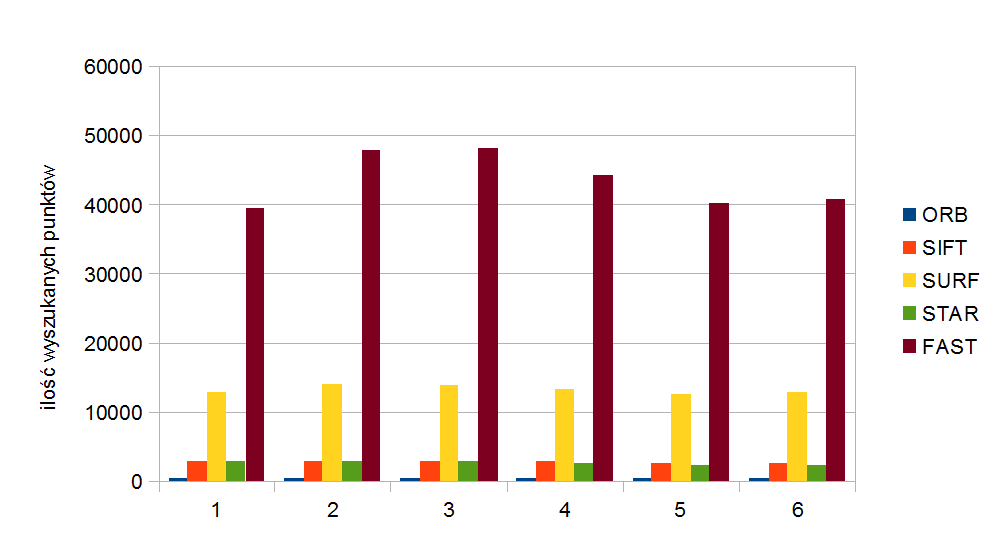
\includegraphics[width=0.8\textwidth]{pict/slowik/r2/f1.png}
\caption{R2 - ilość wyszukanych cech}
\label{fig:r2_f1}
\end{figure}


% Table generated by Excel2LaTeX from sheet 'm.r2 F'
\begin{table}[htbp]
  \centering
  \caption{R2 - czas lokalizowania pojedynczego punktu charakterystycznego w obrazach z zestawu R2}
    \begin{tabular}{|c|c|c|c|c|c|}
    \hline
    obraz & \textbf{ORB} & \textbf{SIFT} & \textbf{SURF} & \textbf{STAR} & \textbf{FAST} \\
    \hline
    -  & [ms] & [ms] & [ms] & [ms] & [ms] \\\hline
    1 & 0,214 & 0,083 & 0,162 & 0,030 & 0,001 \\
    2 & 0,244 & 0,085 & 0,159 & 0,029 & 0,001 \\
    3 & 0,244 & 0,082 & 0,555 & 0,029 & 0,001 \\
    4 & 0,228 & 0,088 & 0,160 & 0,033 & 0,001 \\
    5 & 0,212 & 0,086 & 0,162 & 0,035 & 0,001 \\
    6 & 0,206 & 0,087 & 0,162 & 0,036 & 0,001 \\\hline
    \textbf{średnia} & \textbf{0,225} & \textbf{0,085} & \textbf{0,227} & \textbf{0,032} & \textbf{0,001} \\
    \hline
    \end{tabular}%
  \label{tab:r2_f2}%
\end{table}%


\begin{figure}
\centering
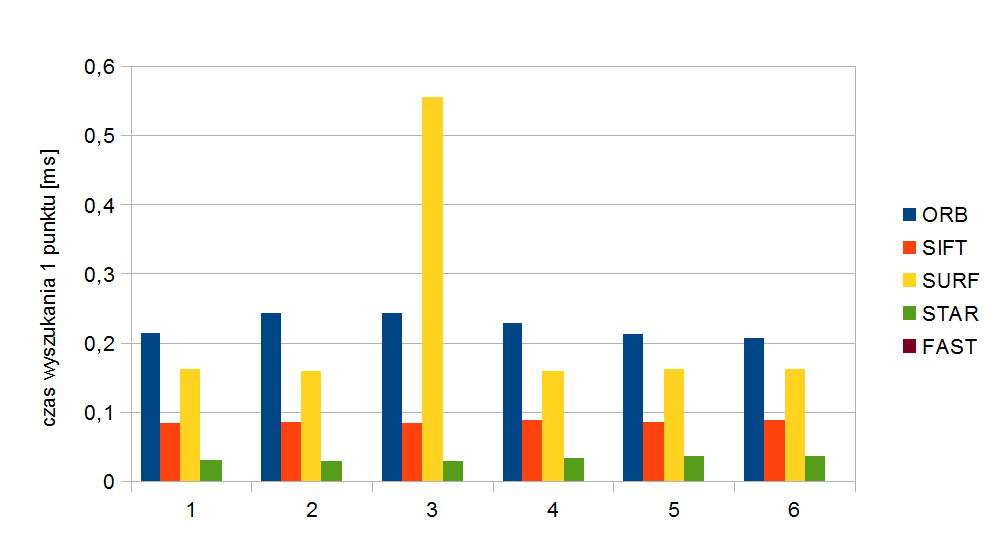
\includegraphics[width=0.8\textwidth]{pict/slowik/r2/f2.png}
\caption{R2 - czas lokalizowania pojedynczego punktu charakterystycznego}
\label{fig:r2_f2}
\end{figure}

% Table generated by Excel2LaTeX from sheet 'm.r2 F'
\begin{table}[htbp]
  \centering
  \caption{R2 - czas generowania pojedynczego deskryptora punktu charakterystycznego}
    \begin{tabular}{|c|c|c|c|c|c|c|c|}\hline

    obraz & \textbf{ORB} & \textbf{SIFT} & \textbf{SURF} & \textbf{ST-BRIEF} & \textbf{ST-ORB} & \textbf{ST-SIFT} & \textbf{ST-SURF} \\\hline

    - & [ms] & [ms] & [ms] & [ms] & [ms] & [ms] & [ms] \\\hline
    1 & 0,100 & 0,215 & 0,202 & 0,012 & 0,012 & 0,709 & 0,089 \\
    2 & 0,102 & 0,217 & 0,196 & 0,012 & 0,012 & 0,678 & 0,089 \\
    3 & 0,100 & 0,213 & 0,192 & 0,012 & 0,012 & 0,702 & 0,089 \\
    4 & 0,100 & 0,221 & 0,192 & 0,012 & 0,012 & 0,773 & 0,090 \\
    5 & 0,102 & 0,219 & 0,192 & 0,012 & 0,012 & 0,733 & 0,090 \\
    6 & 0,100 & 0,221 & 0,195 & 0,012 & 0,012 & 0,690 & 0,089 \\\hline
    \textbf{średnia} & \textbf{0,101} & \textbf{0,218} & \textbf{0,195} & \textbf{0,012} & \textbf{0,012} & \textbf{0,714} & \textbf{0,089} \\\hline
    
    \end{tabular}%
  \label{tab:r2_f3}%
\end{table}%


\begin{figure}
\centering
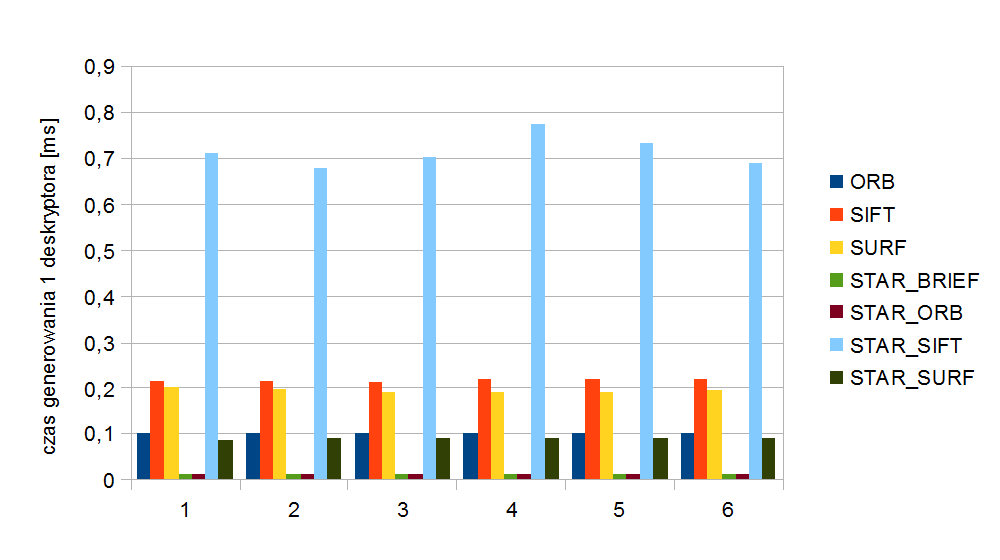
\includegraphics[width=0.8\textwidth]{pict/slowik/r2/f3.png}
\caption{R2 - czas generowania pojedynczego deskryptora punktu charakterystycznego}
\label{fig:r2_f3}
\end{figure}


% Table generated by Excel2LaTeX from sheet 'm.r2 M'
\begin{table}[htbp]
  \centering
  \caption{R2 - powtarzalność wykrywanych cech}
    \begin{tabular}{|c|c|c|c|c|c|c|c|}\hline

    obrazy & \textbf{ORB} & \textbf{SIFT} & \textbf{SURF} & \textbf{ST-BRIEF} & \textbf{ST-ORB} & \textbf{ST-SIFT} & \textbf{ST-SURF} \\\hline

    -  & [\%] & [\%] & [\%] & [\%] & [\%] & [\%] & [\%] \\\hline
    1|2 & 54 & 51 & 16 & 24 & 8 & 43 & 10 \\
    1|3 & 48 & 55 & 12 & 1 & 1 & 0 & 9 \\
    1|4 & 57 & 45 & 14 & 1 & 1 & 0 & 12 \\
    1|5 & 55 & 55 & 16 & 1 & 1 & 0 & 9 \\
    1|6 & 44 & 47 & 12 & 2 & 1 & 0 & 9 \\\hline
    \textbf{średnia} & \textbf{52} & \textbf{51} & \textbf{14} & \textbf{6} & \textbf{2} & \textbf{9} & \textbf{10} \\\hline
    

    \end{tabular}%
  \label{tab:r2_m1}%
\end{table}%


\begin{figure}
\centering
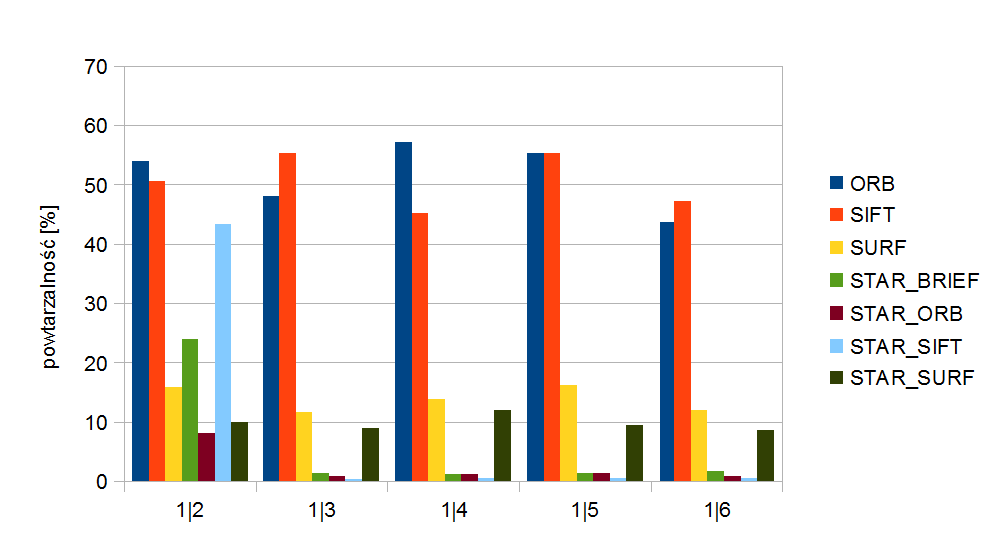
\includegraphics[width=0.8\textwidth]{pict/slowik/r2/m1.png}
\caption{R2 - powtarzalność wykrywanych cech}
\label{fig:r2_m1}
\end{figure}

% Table generated by Excel2LaTeX from sheet 'm.r2 M'
\begin{table}[htbp]
  \centering
  \caption{R2 - procent poprawnych dopasowań}
    \begin{tabular}{|c|c|c|c|c|c|c|c|}\hline
    obrazy & \textbf{ORB} & \textbf{SIFT} & \textbf{SURF} & \textbf{ST-BRIEF} & \textbf{ST-ORB} & \textbf{ST-SIFT} & \textbf{ST-SURF} \\\hline
     - & [\%] & [\%] & [\%] & [\%] & [\%] & [\%] & [\%] \\\hline
    1|2 & 75 & 77 & 39 & 72 & 67 & 82 & 61 \\
    1|3 & 71 & 90 & 49 & 10 & 13 & 33 & 57 \\
    1|4 & 84 & 69 & 49 & 8 & 9 & 24 & 71 \\
    1|5 & 72 & 93 & 60 & 9 & 7 & 33 & 61 \\
    1|6 & 51 & 71 & 32 & 10 & 11 & 20 & 55 \\\hline
    \textbf{średnia} & \textbf{71} & \textbf{80} & \textbf{46} & \textbf{22} & \textbf{22} & \textbf{39} & \textbf{61} \\\hline
    
    \end{tabular}%
  \label{tab:r2_m2}%
\end{table}%


\begin{figure}
\centering
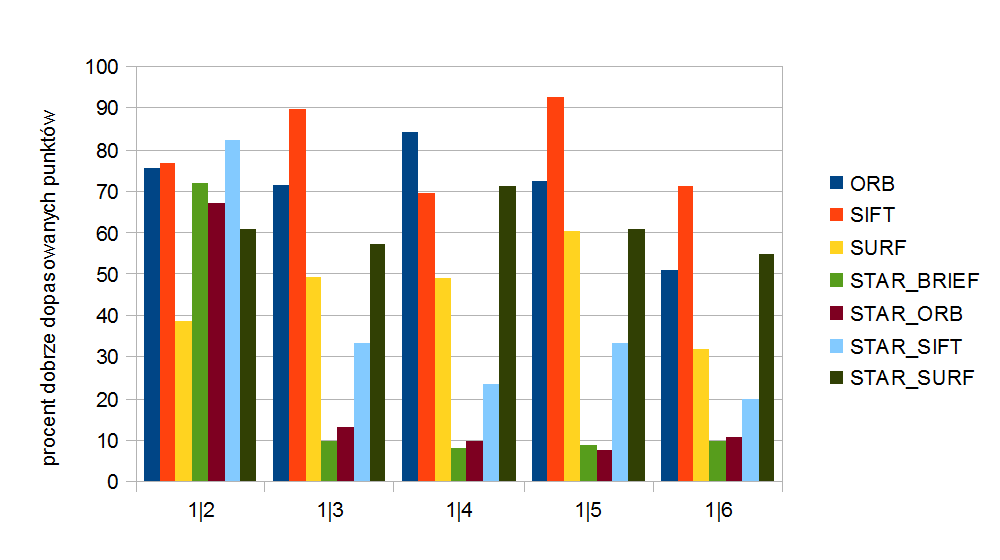
\includegraphics[width=0.8\textwidth]{pict/slowik/r2/m2.png}
\caption{R2 - procent poprawnych dopasowań}
\label{fig:r2_m2}
\end{figure}




\FloatBarrier
\newpage
\subsection{R3}
Transformacja: Rotacja\\
Rejon: Krzywa Turnia\\
Powiększenie: Średnie\\
Oświetlenie: Mieszane\\
Rozdzielczość: $1024 \times 768$\\

\begin{figure}[!htb]
\begin{center}
\subfigure[R3 1]{
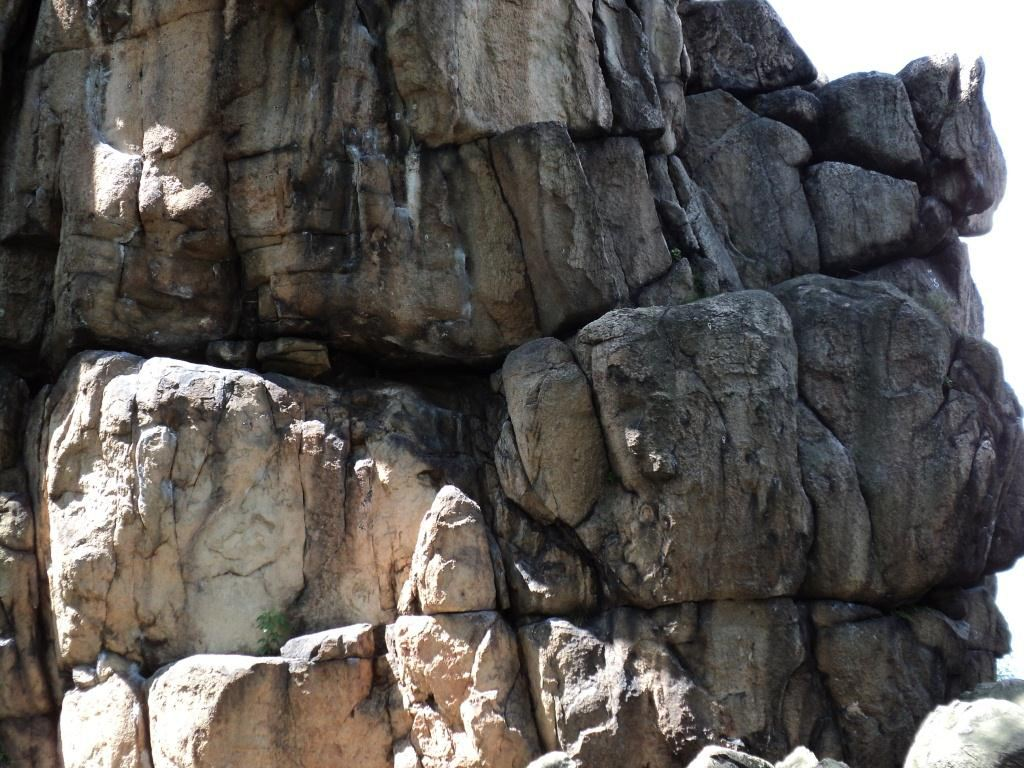
\includegraphics[width=5cm]{pict/slowik/r3/img1.jpg}
}
\subfigure[R3 2]{
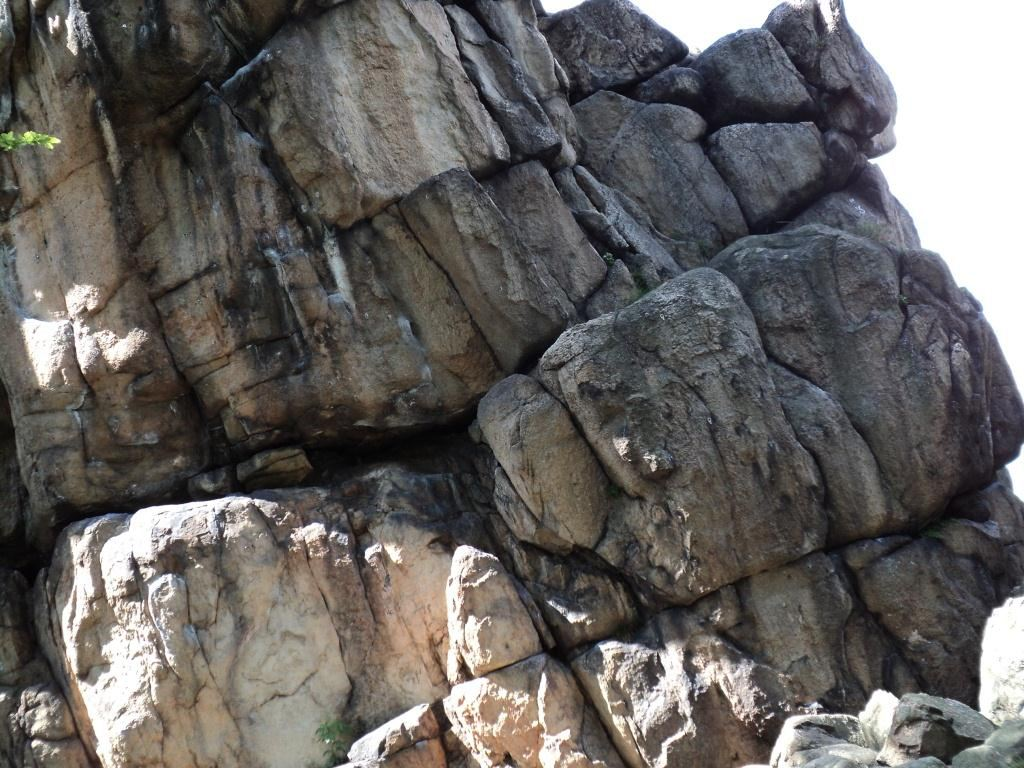
\includegraphics[width=5cm]{pict/slowik/r3/img2.jpg}
}
\subfigure[R3 3]{
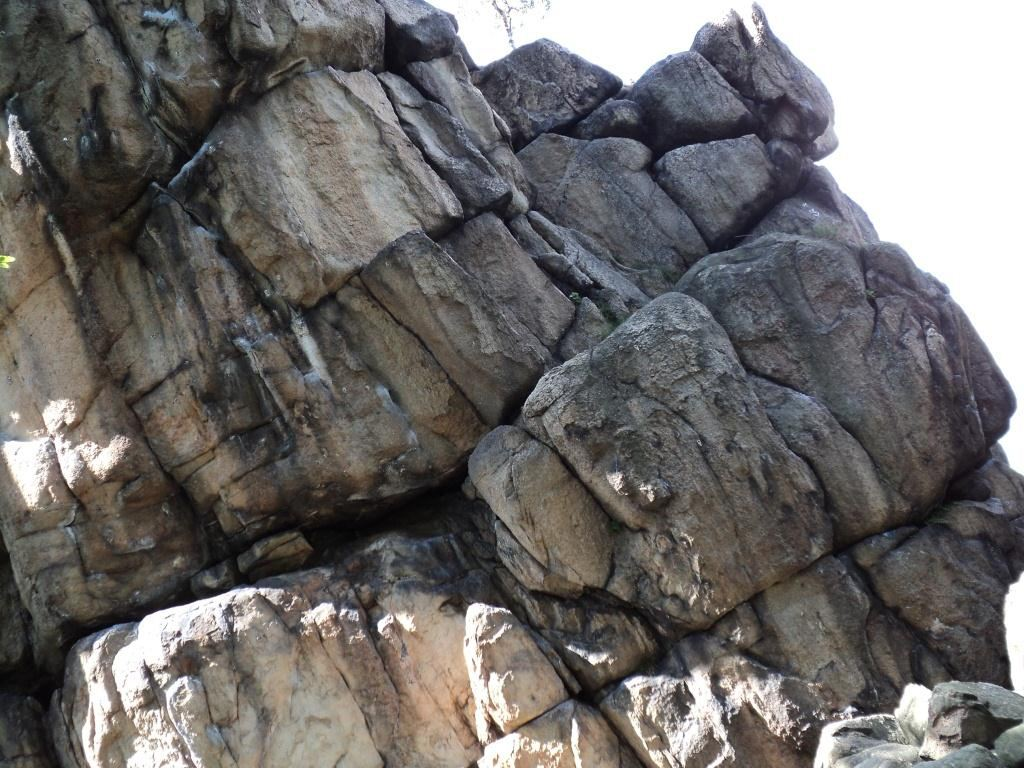
\includegraphics[width=5cm]{pict/slowik/r3/img3.jpg}
}
\subfigure[R3 4]{
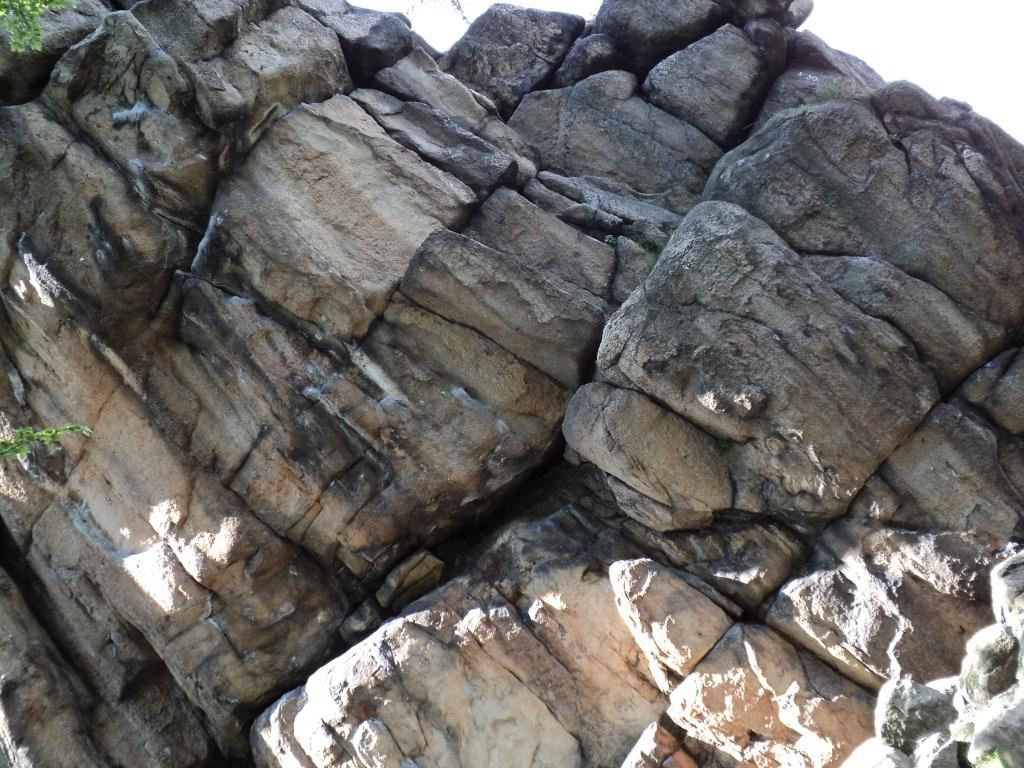
\includegraphics[width=5cm]{pict/slowik/r3/img4.jpg}
}
\subfigure[R3 5]{
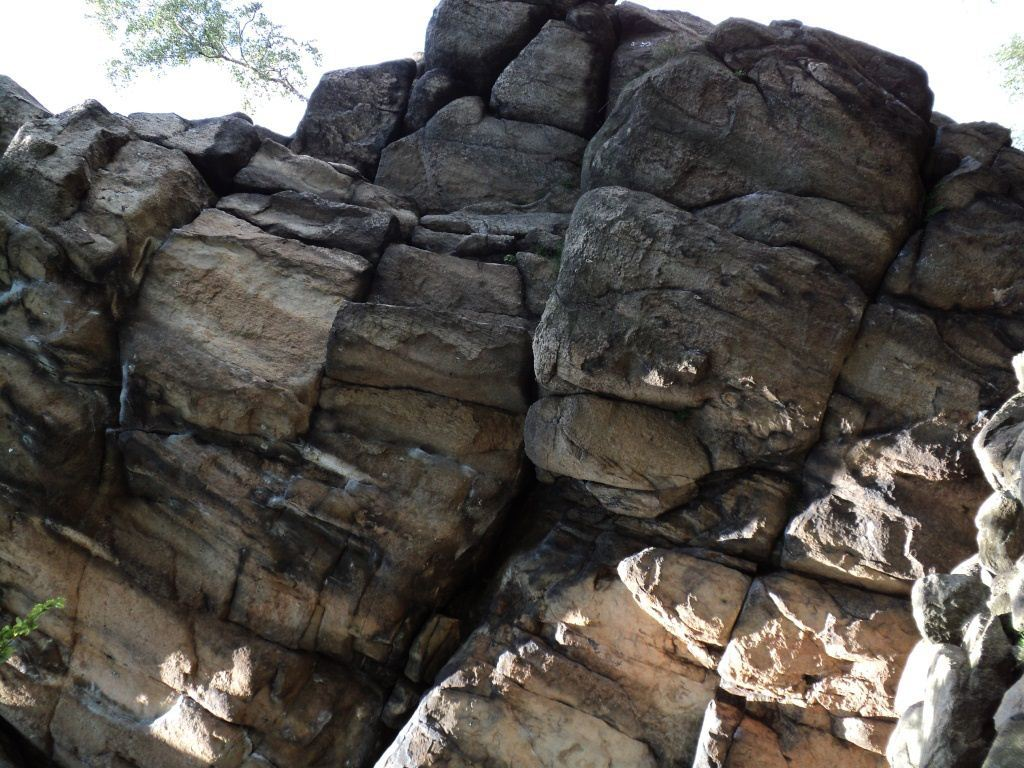
\includegraphics[width=5cm]{pict/slowik/r3/img5.jpg}
}
\subfigure[R3 6]{
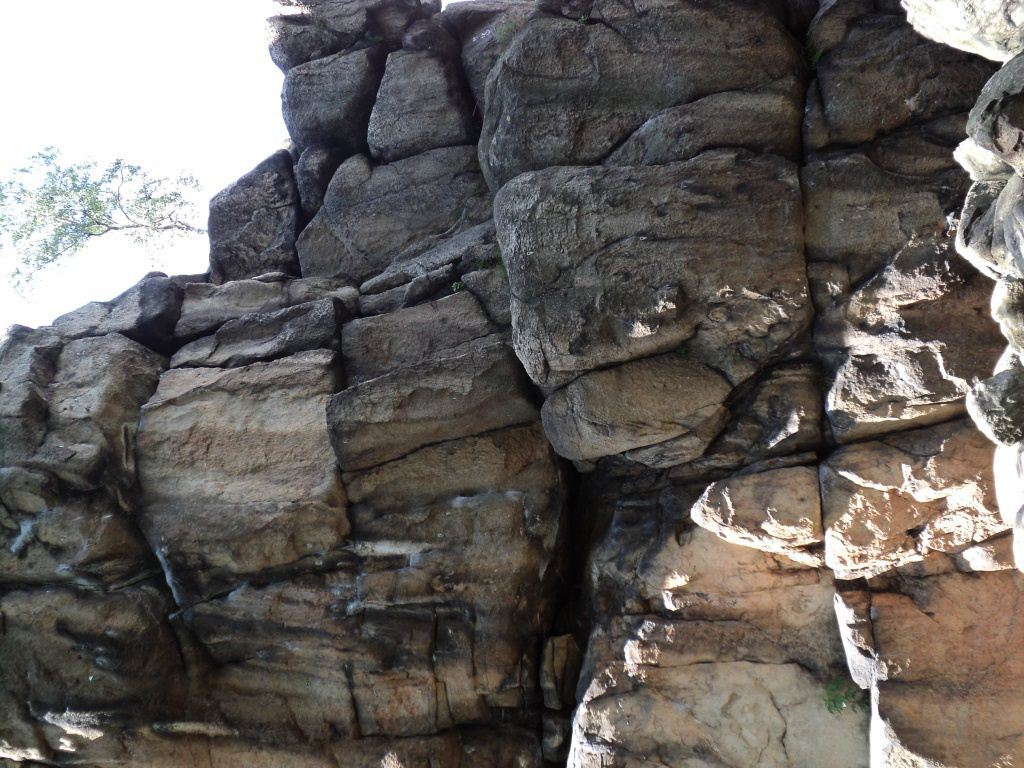
\includegraphics[width=5cm]{pict/slowik/r3/img6.jpg}
}
\caption{R3 - zbiór obrazów testowych}
\label{fig:r3_set}
\end{center}
\end{figure}



% Table generated by Excel2LaTeX from sheet 'm.r3 F'
\begin{table}[htbp]
  \centering
  \caption{R3 - ilość wyszukanych cech}
    \begin{tabular}{|c|r|r|r|r|r|}\hline
    
    obraz & \textbf{ORB} & \textbf{SIFT} & \textbf{SURF} & \textbf{STAR} & \textbf{FAST} \\\hline
    
    1 & 500 & 1847 & 10957 & 690 & 18567 \\
    2 & 500 & 2021 & 10701 & 686 & 20103 \\
    3 & 500 & 2054 & 10452 & 579 & 21226 \\
    4 & 500 & 2413 & 10839 & 785 & 24483 \\
    5 & 500 & 1787 & 10631 & 653 & 18969 \\
    6 & 500 & 1869 & 10903 & 722 & 20906 \\\hline
    \textbf{średnia} & \textbf{500} & \textbf{1999} & \textbf{10747} & \textbf{686} & \textbf{20709} \\
    \hline
    \end{tabular}%
  \label{tab:r3_f1}%
\end{table}%


\begin{figure}
\centering
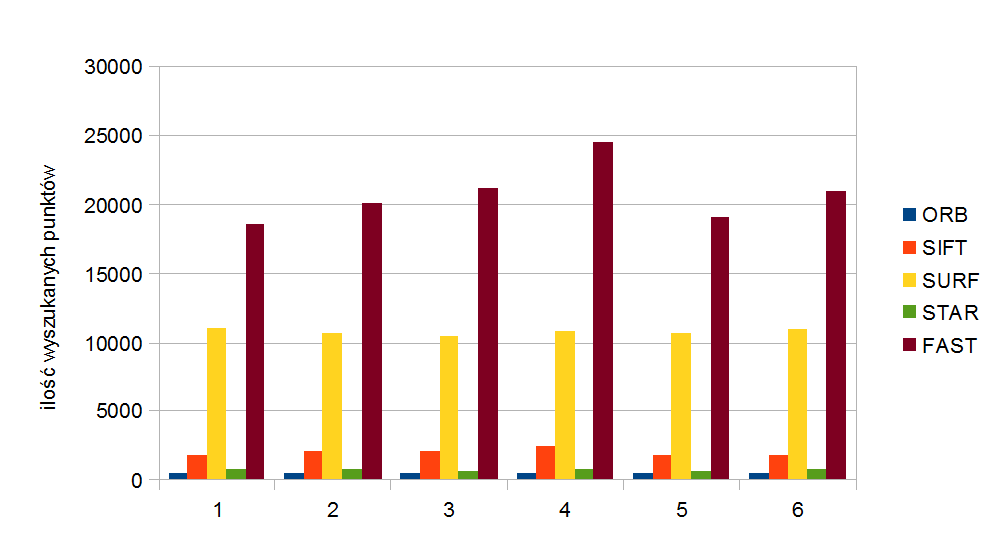
\includegraphics[width=0.8\textwidth]{pict/slowik/r3/f1.png}
\caption{R3 - ilość wyszukanych cech}
\label{fig:r3_f1}
\end{figure}


% Table generated by Excel2LaTeX from sheet 'm.r3 F'
\begin{table}[htbp]
  \centering
  \caption{R3 - czas lokalizowania pojedynczego punktu charakterystycznego}
    \begin{tabular}{|c|c|c|c|c|c|}
    \hline
    obraz & \textbf{ORB} & \textbf{SIFT} & \textbf{SURF} & \textbf{STAR} & \textbf{FAST} \\
    \hline
    -  & [ms] & [ms] & [ms] & [ms] & [ms] \\\hline
    1 & 0,110 & 0,122 & 0,172 & 0,126 & 0,001 \\
    2 & 0,122 & 0,113 & 0,172 & 0,125 & 0,001 \\
    3 & 0,116 & 0,111 & 0,173 & 0,149 & 0,001 \\
    4 & 0,128 & 0,101 & 0,171 & 0,111 & 0,001 \\
    5 & 0,112 & 0,128 & 0,173 & 0,132 & 0,001 \\
    6 & 0,112 & 0,121 & 0,171 & 0,120 & 0,001 \\\hline
    \textbf{średnia} & \textbf{0,117} & \textbf{0,116} & \textbf{0,172} & \textbf{0,127} & \textbf{0,001} \\
    \hline
    \end{tabular}%
  \label{tab:r3_f2}%
\end{table}%


\begin{figure}
\centering
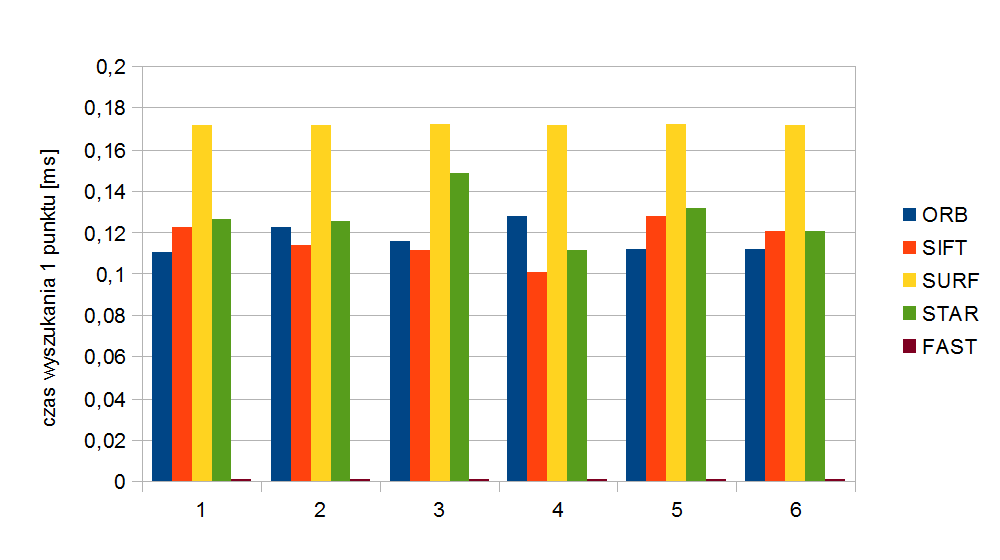
\includegraphics[width=0.8\textwidth]{pict/slowik/r3/f2.png}
\caption{R3 - czas lokalizowania pojedynczego punktu charakterystycznego}
\label{fig:r3_f2}
\end{figure}

% Table generated by Excel2LaTeX from sheet 'm.r3 F'
\begin{table}[htbp]
  \centering
  \caption{R3 - czas generowania pojedynczego deskryptora punktu charakterystycznego}
    \begin{tabular}{|c|c|c|c|c|c|c|c|}\hline

    obraz & \textbf{ORB} & \textbf{SIFT} & \textbf{SURF} & \textbf{ST-BRIEF} & \textbf{ST-ORB} & \textbf{ST-SIFT} & \textbf{ST-SURF} \\\hline

    - & [ms] & [ms] & [ms] & [ms] & [ms] & [ms] & [ms] \\\hline
    1 & 0,102 & 0,254 & 0,198 & 0,020 & 0,019 & 1,462 & 0,106 \\
    2 & 0,104 & 0,243 & 0,193 & 0,020 & 0,019 & 1,443 & 0,106 \\
    3 & 0,100 & 0,243 & 0,196 & 0,022 & 0,021 & 1,577 & 0,109 \\
    4 & 0,100 & 0,234 & 0,193 & 0,020 & 0,018 & 1,367 & 0,104 \\
    5 & 0,100 & 0,259 & 0,191 & 0,021 & 0,020 & 1,424 & 0,106 \\
    6 & 0,100 & 0,252 & 0,198 & 0,021 & 0,019 & 1,385 & 0,105 \\\hline
    \textbf{średnia} & \textbf{0,101} & \textbf{0,247} & \textbf{0,195} & \textbf{0,021} & \textbf{0,019} & \textbf{1,443} & \textbf{0,106} \\\hline
    
    \end{tabular}%
  \label{tab:r3_f3}%
\end{table}%


\begin{figure}
\centering
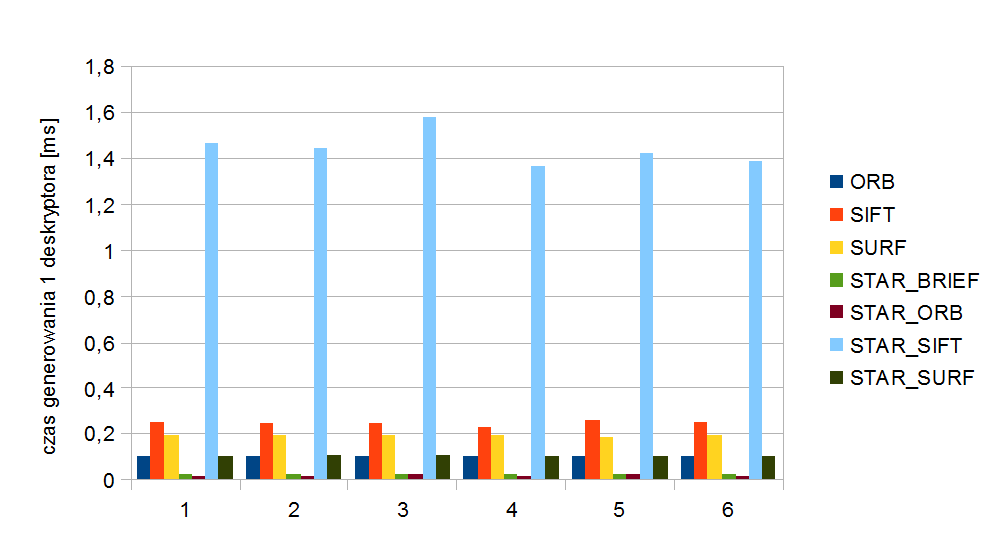
\includegraphics[width=0.8\textwidth]{pict/slowik/r3/f3.png}
\caption{R3 - czas generowania pojedynczego deskryptora punktu charakterystycznego}
\label{fig:r3_f3}
\end{figure}


% Table generated by Excel2LaTeX from sheet 'm.r3 M'
\begin{table}[htbp]
  \centering
  \caption{R3 - powtarzalność wykrywanych cech dla obrazów z zestawu R3}
    \begin{tabular}{|c|c|c|c|c|c|c|c|}\hline

    obrazy & \textbf{ORB} & \textbf{SIFT} & \textbf{SURF} & \textbf{ST-BRIEF} & \textbf{ST-ORB} & \textbf{ST-SIFT} & \textbf{ST-SURF} \\\hline

    -  & [\%] & [\%] & [\%] & [\%] & [\%] & [\%] & [\%] \\\hline
    1|2 & 53 & 54 & 25 & 19 & 7 & 28 & 20 \\
    1|3 & 36 & 44 & 20 & 2 & 2 & 1 & 11 \\
    1|4 & 36 & 44 & 17 & 4 & 2 & 1 & 14 \\
    1|5 & 37 & 46 & 19 & 1 & 3 & 1 & 14 \\
    1|6 & 38 & 50 & 35 & 2 & 2 & 1 & 23 \\\hline
    \textbf{średnia} & \textbf{40} & \textbf{47} & \textbf{23} & \textbf{6} & \textbf{3} & \textbf{6} & \textbf{16} \\
    

    \end{tabular}%
  \label{tab:r3_m1}%
\end{table}%


\begin{figure}
\centering
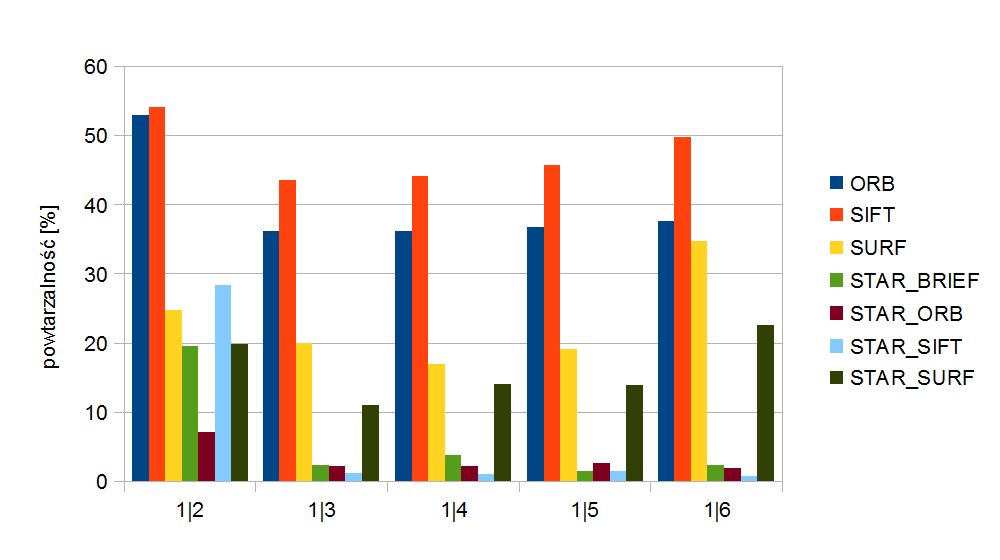
\includegraphics[width=0.8\textwidth]{pict/slowik/r3/m1.png}
\caption{R3 - powtarzalność wykrywanych cech}
\label{fig:r3_m1}
\end{figure}

% Table generated by Excel2LaTeX from sheet 'm.r3 M'
\begin{table}[htbp]
  \centering
  \caption{R3 - procent poprawnych dopasowań}
    \begin{tabular}{|c|c|c|c|c|c|c|c|}\hline
    obrazy & \textbf{ORB} & \textbf{SIFT} & \textbf{SURF} & \textbf{ST-BRIEF} & \textbf{ST-ORB} & \textbf{ST-SIFT} & \textbf{ST-SURF} \\\hline
     - & [\%] & [\%] & [\%] & [\%] & [\%] & [\%] & [\%] \\\hline
    1|2 & 79 & 90 & 51 & 70 & 59 & 73 & 50 \\
    1|3 & 65 & 66 & 41 & 18 & 17 & 36 & 55 \\
    1|4 & 72 & 67 & 46 & 16 & 16 & 57 & 54 \\
    1|5 & 54 & 80 & 48 & 14 & 13 & 36 & 47 \\
    1|6 & 69 & 82 & 48 & 18 & 14 & 57 & 76 \\\hline
    \textbf{średnia} & \textbf{68} & \textbf{77} & \textbf{47} & \textbf{27} & \textbf{24} & \textbf{52} & \textbf{56} \\\hline
    
    \end{tabular}%
  \label{tab:r3_m2}%
\end{table}%


\begin{figure}
\centering
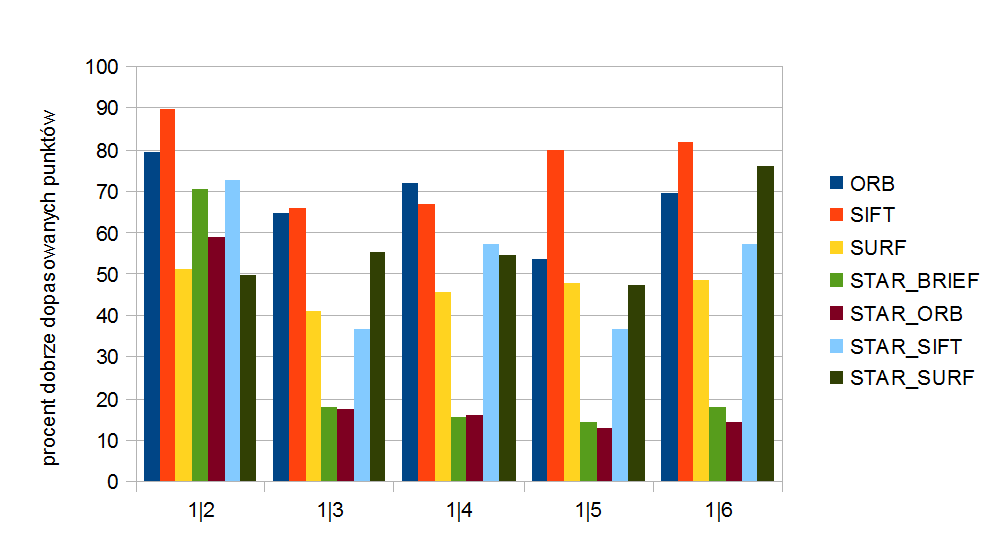
\includegraphics[width=0.8\textwidth]{pict/slowik/r3/m2.png}
\caption{R3 - procent poprawnych dopasowań}
\label{fig:r3_m2}
\end{figure}


\FloatBarrier
\subsection{Dyskusja wyników}
Dla przygotowanych zbiorów wszystkie algorytmy wykazują stabilność wskaźników takich jak ilość generowanych lokalizowanych punktów i charakterystyki czasowe. Tradycjnie o algorytm FAST lokalizuje o rząd wielkości więcej punktów, kolejne w kolejności są algorytmy SURF, SIFT, STAR i ograniczony parametrycznie ORB.

Czasy lokalizowania punktu przes FAST są również znikomo małe. W zależności od badanej sceny czas lokalizowania przez algorytm ORB może zmieniać się o blisko 100\%. Algorytm ten spowalnia dla obrazów o dużym stopniu przybliżenia. Prawdopodobnie spowodowane dużą szczegółowością obrazów, a co za tym idzie dużą liczbą zgrubnych punktów charakterystycznych, które trzeba ocenić miarą Harrisa. Na tle tych charaktestyk czasowych najlepsze wyniki osiąga algorytm STAR.

Czas generowania deskryptora można uznać za stały niezależnie od typu obrazów. Podobnie jak w badaniach dla zbioru Mikołajczyka kombinacja STAR-SIFT jest w sposób radykalny najwolniejszą w tej kategorii.

Badając powtarzalność algorytmów możemy zaobserwować większe zróżnicowanie w wynikach. W tej dziedzinie jako wiodące możemy uznać algorytmy ORB i SIFT. Dla obrazów o dużym stopniu przybliżenia ich wyniki są niemal równe. Większość algorytmów dobrze radzi sobie z niewielkim stopniem rotacji obrazu przy dużym powiększeniu Jakość ich jednak spada w sposób znaczący przy większych kątach obrotu. Najlepsze wyniki na tym polu osiągają algorytmy ORB i SIFT, których minimum wyników przypada w okolicach kąta $45^o$.

Najkorzystniejszy współczynnik poprawnych dopasowań posiada algorytm SIFT. Dobre wyniki osiągają również wyniki dla algorytmów ORB i STAR-SURF. Przewaga algorytmu SIFT ujawnia się w kątach powyżej $60^o$. Pozostałe metody dla większych kątów osiągają wskaźnik poprawności poniżej 50 \%.





\FloatBarrier
\newpage
\section{Zmiana położenia obserwatora}
\FloatBarrier
\subsection{V1}
Transformacja: Zmiana położenia obserwatora\\
Rejon: Mały Sokolik\\
Powiększenie: Duże\\
Oświetlenie: Duże\\
Rozdzielczość: $585 \times 1024$

\begin{figure}[!htb]
\begin{center}
\subfigure[V1 1]{
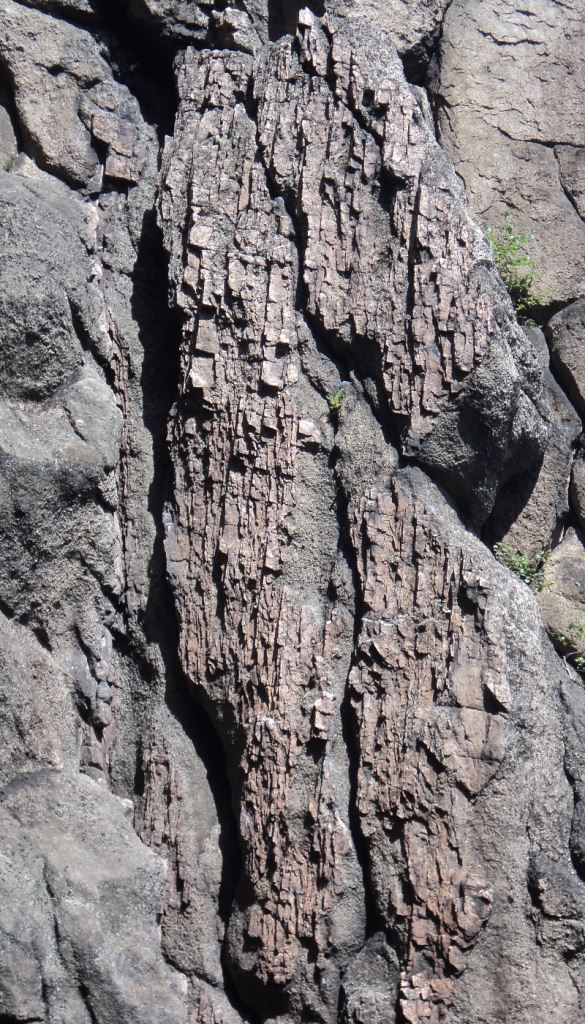
\includegraphics[height=6cm]{pict/slowik/v1/img1.jpg}
}
\subfigure[V1 2]{
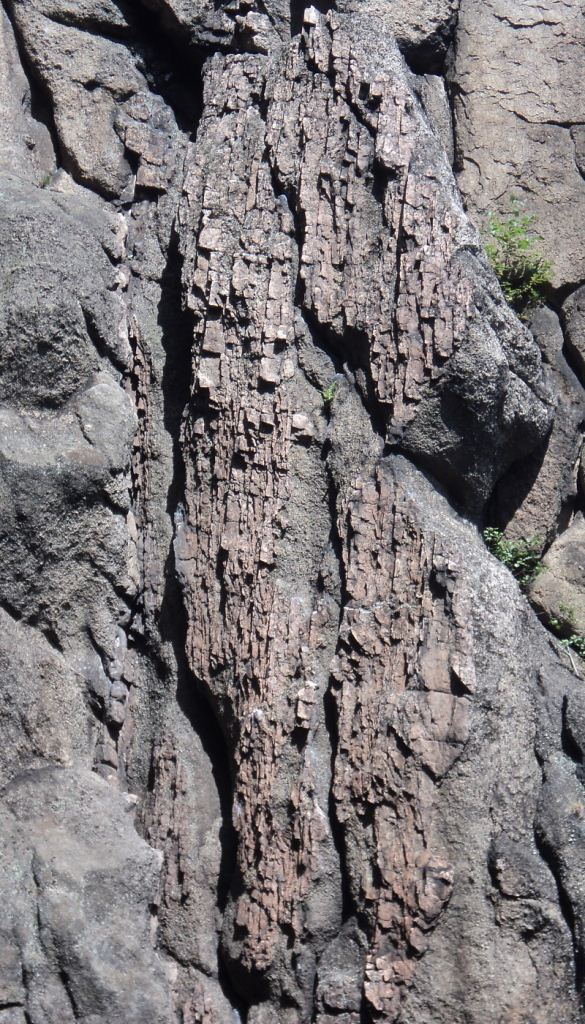
\includegraphics[height=6cm]{pict/slowik/v1/img2.jpg}
}
\subfigure[V1 3]{
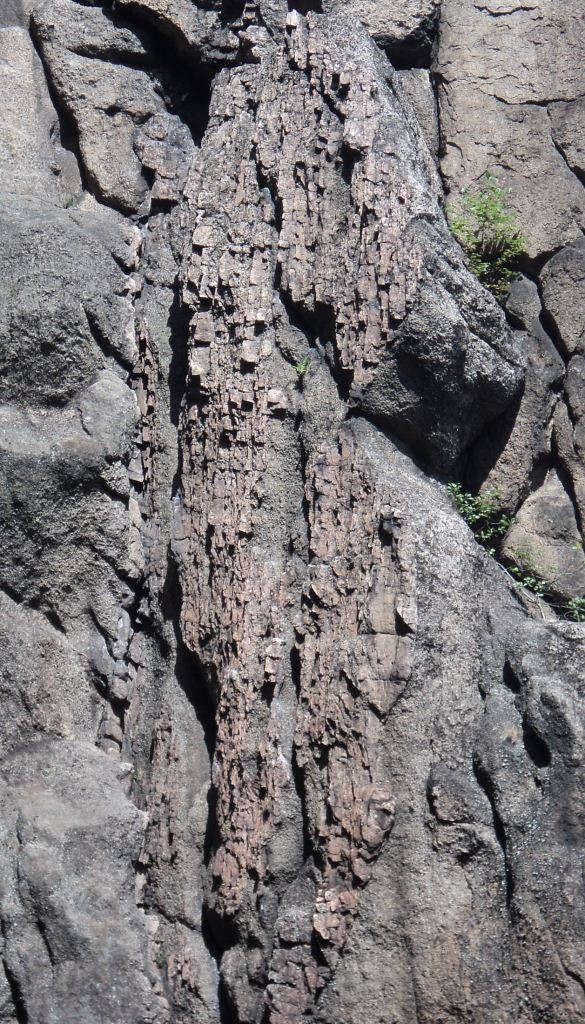
\includegraphics[height=6cm]{pict/slowik/v1/img3.jpg}
}\\
\subfigure[V1 4]{
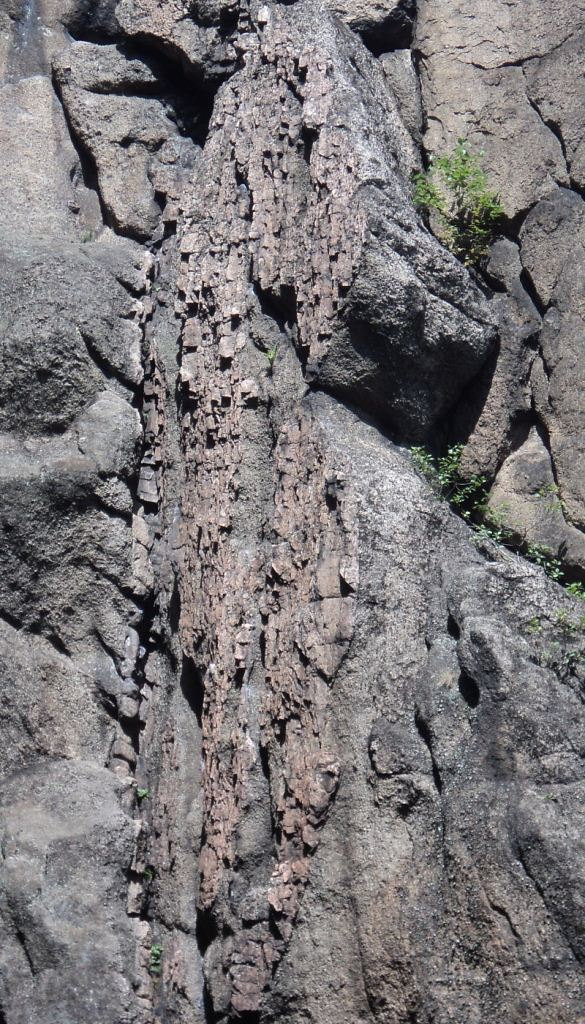
\includegraphics[height=6cm]{pict/slowik/v1/img4.jpg}
}
\subfigure[V1 5]{
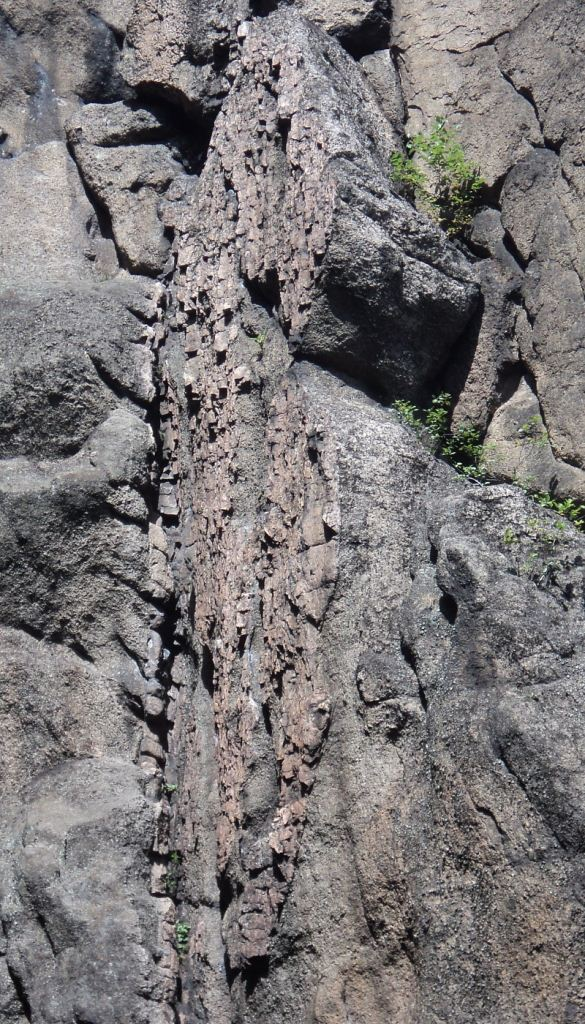
\includegraphics[height=6cm]{pict/slowik/v1/img5.jpg}
}
\subfigure[V1 6]{
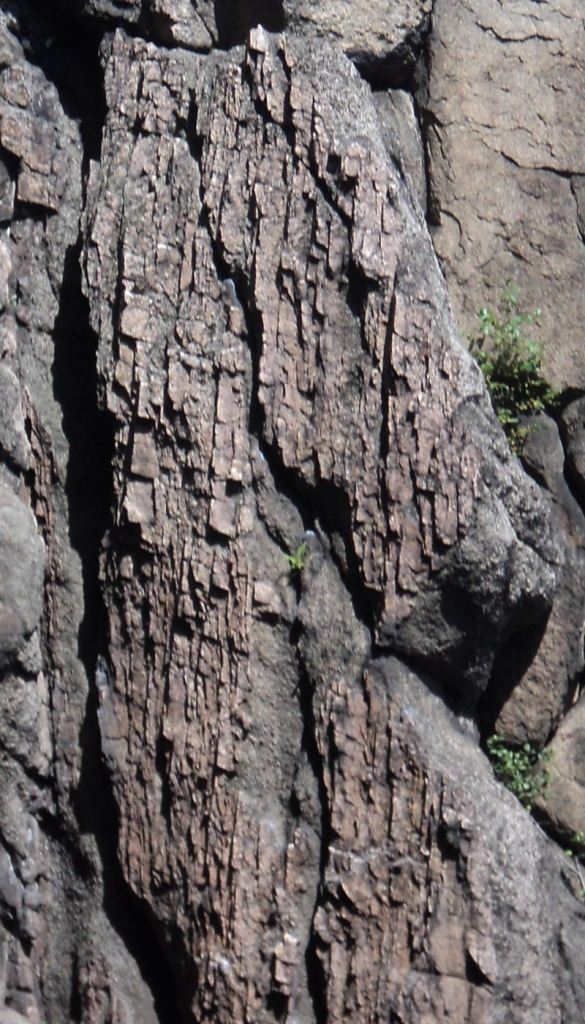
\includegraphics[height=6cm]{pict/slowik/v1/img6.jpg}
}
\caption{V1 - zbiór obrazów testowych}
\label{fig:v1_set}
\end{center}
\end{figure}



% Table generated by Excel2LaTeX from sheet 'm.v1 F'
\begin{table}[htbp]
  \centering
  \caption{V1 - ilość wyszukanych cech}
    \begin{tabular}{|c|r|r|r|r|r|}\hline
    
    obraz & \textbf{ORB} & \textbf{SIFT} & \textbf{SURF} & \textbf{STAR} & \textbf{FAST} \\\hline
    
  
    1 & 500 & 2463 & 10032 & 2951 & 34032 \\
    2 & 500 & 2472 & 9698 & 2601 & 33659 \\
    3 & 500 & 2317 & 10096 & 2344 & 35807 \\
    4 & 500 & 2125 & 9966 & 2133 & 35498 \\
    5 & 500 & 2106 & 10194 & 2032 & 36830 \\
    6 & 500 & 2844 & 8021 & 2562 & 21418 \\\hline
    \textbf{średnia} & \textbf{500} & \textbf{2388} & \textbf{9668} & \textbf{2437} & \textbf{32874} \\
    \hline
    \end{tabular}%
  \label{tab:v1_f1}%
\end{table}%


\begin{figure}
\centering
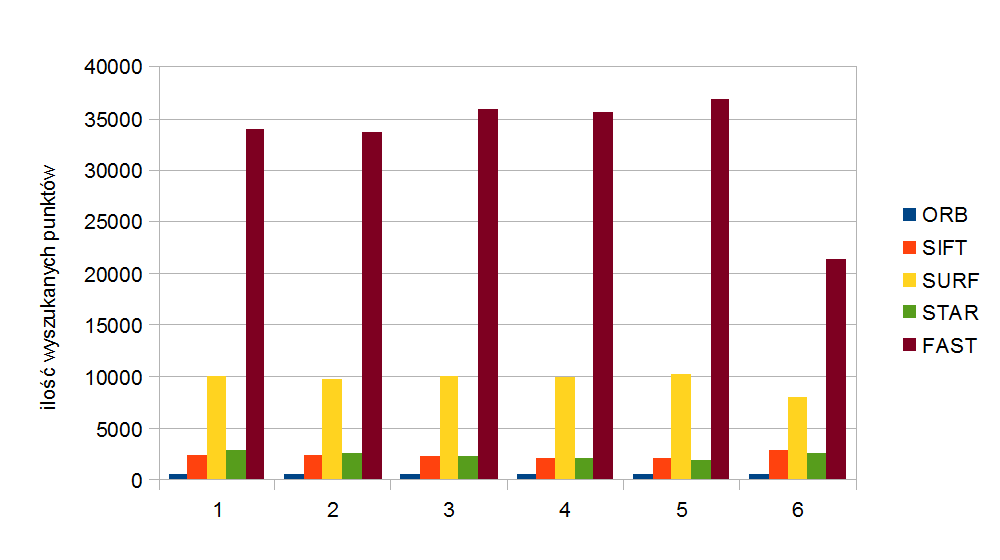
\includegraphics[width=0.8\textwidth]{pict/slowik/v1/f1.png}
\caption{V1 - ilość wyszukanych cech}
\label{fig:v1_f1}
\end{figure}


% Table generated by Excel2LaTeX from sheet 'm.v1 F'
\begin{table}[htbp]
  \centering
  \caption{V1 - czas lokalizowania pojedynczego punktu charakterystycznego}
    \begin{tabular}{|c|c|c|c|c|c|}
    \hline
    obraz & \textbf{ORB} & \textbf{SIFT} & \textbf{SURF} & \textbf{STAR} & \textbf{FAST} \\
    \hline
    -  & [ms] & [ms] & [ms] & [ms] & [ms] \\\hline
    1 & 0,192 & 0,076 & 0,160 & 0,019 & 0,001 \\
    2 & 0,188 & 0,076 & 0,161 & 0,021 & 0,001 \\
    3 & 0,190 & 0,080 & 0,160 & 0,023 & 0,001 \\
    4 & 0,186 & 0,085 & 0,161 & 0,025 & 0,001 \\
    5 & 0,190 & 0,086 & 0,160 & 0,027 & 0,001 \\
    6 & 0,156 & 0,069 & 0,168 & 0,021 & 0,001 \\\hline
    \textbf{średnia} & \textbf{0,184} & \textbf{0,079} & \textbf{0,162} & \textbf{0,023} & \textbf{0,001} \\
    \hline
    \end{tabular}%
  \label{tab:v1_f2}%
\end{table}%


\begin{figure}
\centering
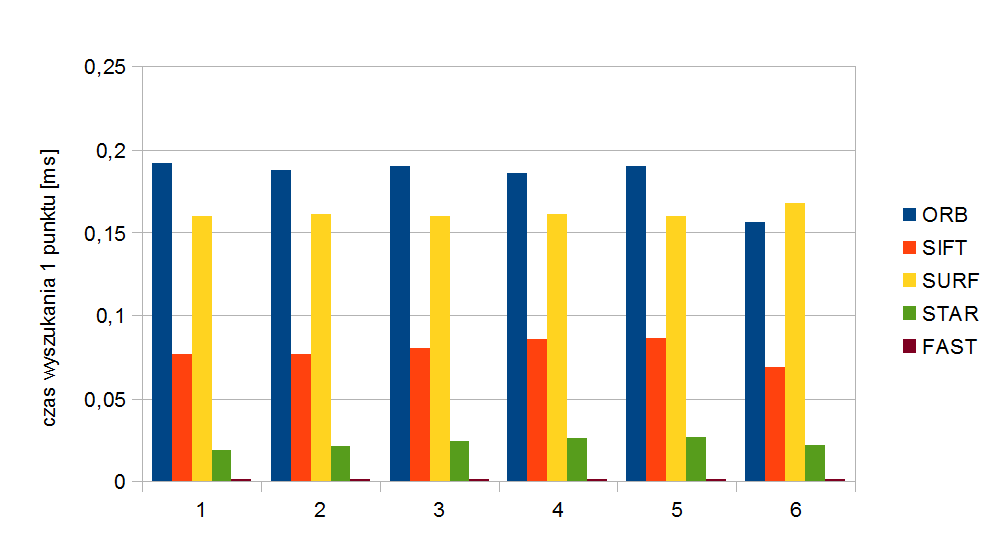
\includegraphics[width=0.8\textwidth]{pict/slowik/v1/f2.png}
\caption{V1 - czas lokalizowania pojedynczego punktu charakterystycznego}
\label{fig:v1_f2}
\end{figure}

% Table generated by Excel2LaTeX from sheet 'm.v1 F'
\begin{table}[htbp]
  \centering
  \caption{V1 - czas generowania pojedynczego deskryptora punktu charakterystycznego}
    \begin{tabular}{|c|c|c|c|c|c|c|c|}\hline

    obraz & \textbf{ORB} & \textbf{SIFT} & \textbf{SURF} & \textbf{ST-BRIEF} & \textbf{ST-ORB} & \textbf{ST-SIFT} & \textbf{ST-SURF} \\\hline

    - & [ms] & [ms] & [ms] & [ms] & [ms] & [ms] & [ms] \\\hline
    1 & 0,082 & 0,213 & 0,201 & 0,011 & 0,011 & 0,688 & 0,088 \\
    2 & 0,082 & 0,211 & 0,201 & 0,012 & 0,011 & 0,665 & 0,088 \\
    3 & 0,082 & 0,216 & 0,196 & 0,012 & 0,012 & 0,684 & 0,089 \\
    4 & 0,082 & 0,223 & 0,196 & 0,012 & 0,012 & 0,737 & 0,090 \\
    5 & 0,082 & 0,221 & 0,197 & 0,012 & 0,012 & 0,742 & 0,090 \\
    6 & 0,082 & 0,206 & 0,214 & 0,011 & 0,011 & 0,651 & 0,085 \\\hline
    \textbf{średnia} & \textbf{0,082} & \textbf{0,215} & \textbf{0,201} & \textbf{0,012} & \textbf{0,011} & \textbf{0,694} & \textbf{0,088} \\\hline
    

    \end{tabular}%
  \label{tab:v1_f3}%
\end{table}%


\begin{figure}
\centering
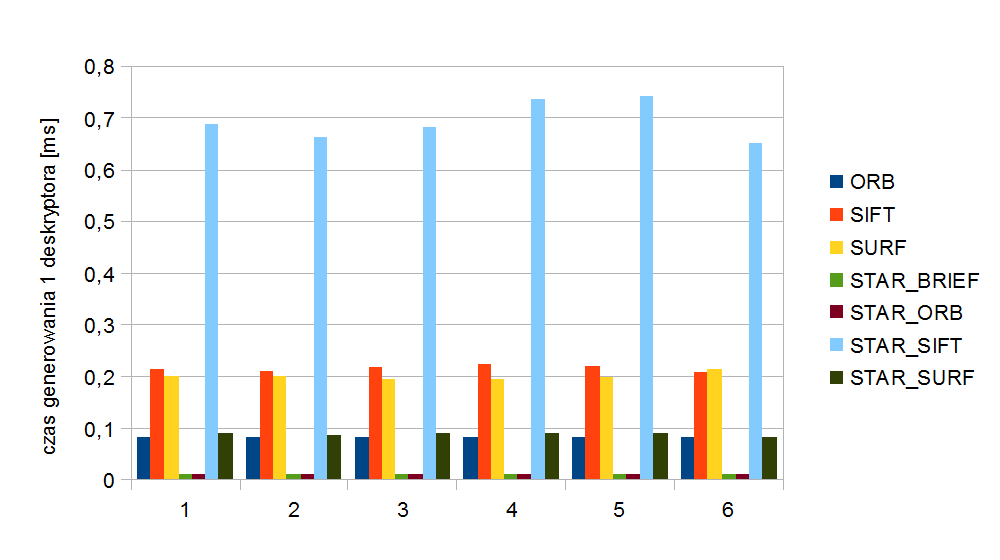
\includegraphics[width=0.8\textwidth]{pict/slowik/v1/f3.png}
\caption{V1 - czas generowania pojedynczego deskryptora punktu charakterystycznego}
\label{fig:v1_f3}
\end{figure}


% Table generated by Excel2LaTeX from sheet 'm.v1 M'
\begin{table}[htbp]
  \centering
  \caption{V1 - powtarzalność wykrywanych cech}
    \begin{tabular}{|c|c|c|c|c|c|c|c|}\hline

    obrazy & \textbf{ORB} & \textbf{SIFT} & \textbf{SURF} & \textbf{ST-BRIEF} & \textbf{ST-ORB} & \textbf{ST-SIFT} & \textbf{ST-SURF} \\\hline

    -  & [\%] & [\%] & [\%] & [\%] & [\%] & [\%] & [\%] \\\hline
    1|2 & 29 & 40 & 26 & 51 & 48 & 53 & 11 \\
    1|3 & 3 & 11 & 5 & 13 & 11 & 16 & 2 \\
    1|4 & 1 & 5 & 2 & 3 & 3 & 4 & 1 \\
    1|5 & 1 & 3 & 1 & 1 & 1 & 1 & 1 \\
    1|6 & 17 & 17 & 8 & 26 & 11 & 41 & 3 \\\hline
    \textbf{średnia} & \textbf{10} & \textbf{15} & \textbf{8} & \textbf{19} & \textbf{15} & \textbf{23} & \textbf{4} \\\hline
   

    \end{tabular}%
  \label{tab:v1_m1}%
\end{table}%


\begin{figure}
\centering
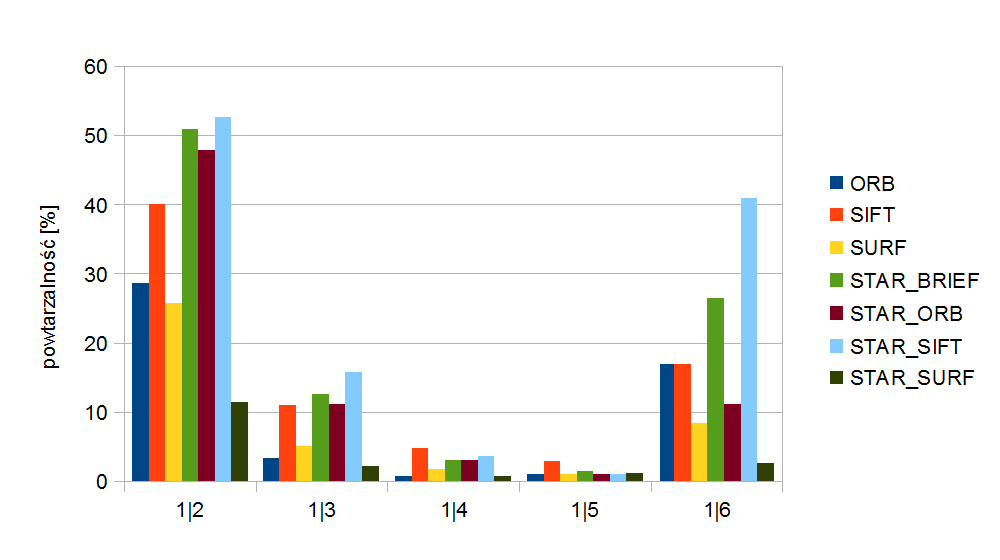
\includegraphics[width=0.8\textwidth]{pict/slowik/v1/m1.png}
\caption{V1 - powtarzalność wykrywanych cech}
\label{fig:v1_m1}
\end{figure}

% Table generated by Excel2LaTeX from sheet 'm.v1 M'
\begin{table}[htbp]
  \centering
  \caption{V1 - procent poprawnych dopasowań}
    \begin{tabular}{|c|c|c|c|c|c|c|c|}\hline
    obrazy & \textbf{ORB} & \textbf{SIFT} & \textbf{SURF} & \textbf{ST-BRIEF} & \textbf{ST-ORB} & \textbf{ST-SIFT} & \textbf{ST-SURF} \\\hline
     - & [\%] & [\%] & [\%] & [\%] & [\%] & [\%] & [\%] \\\hline
    1|2 & 56 & 34 & 29 & 42 & 48 & 43 & 46 \\
    1|3 & 38 & 8 & 7 & 18 & 24 & 22 & 8 \\
    1|4 & 0 & 11 & 4 & 9 & 10 & 12 & 4 \\
    1|5 & 44 & 17 & 4 & 8 & 11 & 24 & 6 \\
    1|6 & 57 & 32 & 23 & 44 & 36 & 55 & 19 \\\hline
    \textbf{średnia} & \textbf{39} & \textbf{20} & \textbf{13} & \textbf{24} & \textbf{26} & \textbf{31} & \textbf{17} \\\hline
   
    \end{tabular}%
  \label{tab:v1_m2}%
\end{table}%


\begin{figure}
\centering
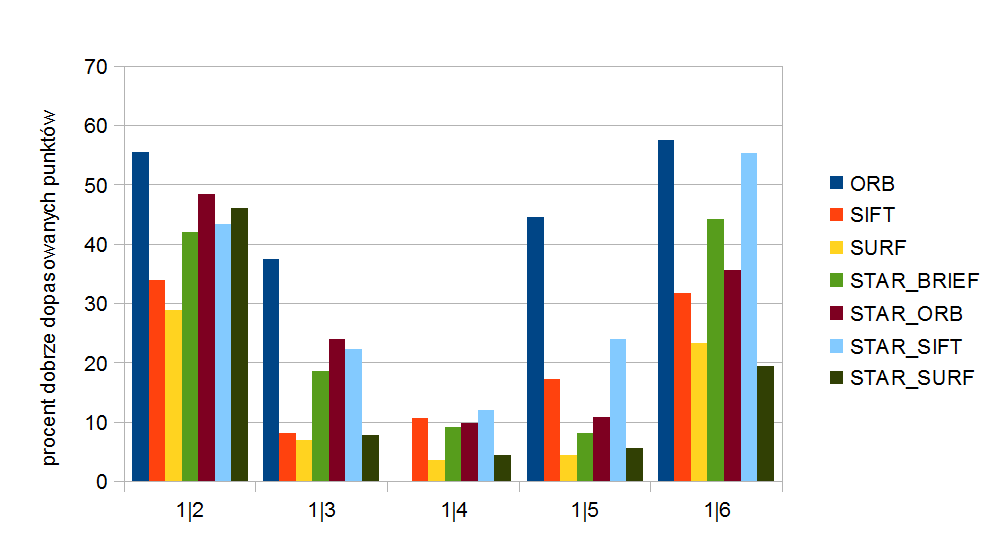
\includegraphics[width=0.8\textwidth]{pict/slowik/v1/m2.png}
\caption{V1 - procent poprawnych dopasowań}
\label{fig:v1_m2}
\end{figure}




\FloatBarrier
\newpage
\subsection{V2}
\FloatBarrier
Transformacja: Zmiana położenia obserwatora\\
Rejon: Signum\\
Powiększenie: Średnie\\
Oświetlenie: Umiarkowane\\
Rozdzielczość: $1024 \times 768$\\
\begin{figure}[!htb]
\begin{center}
\subfigure[V2 1]{
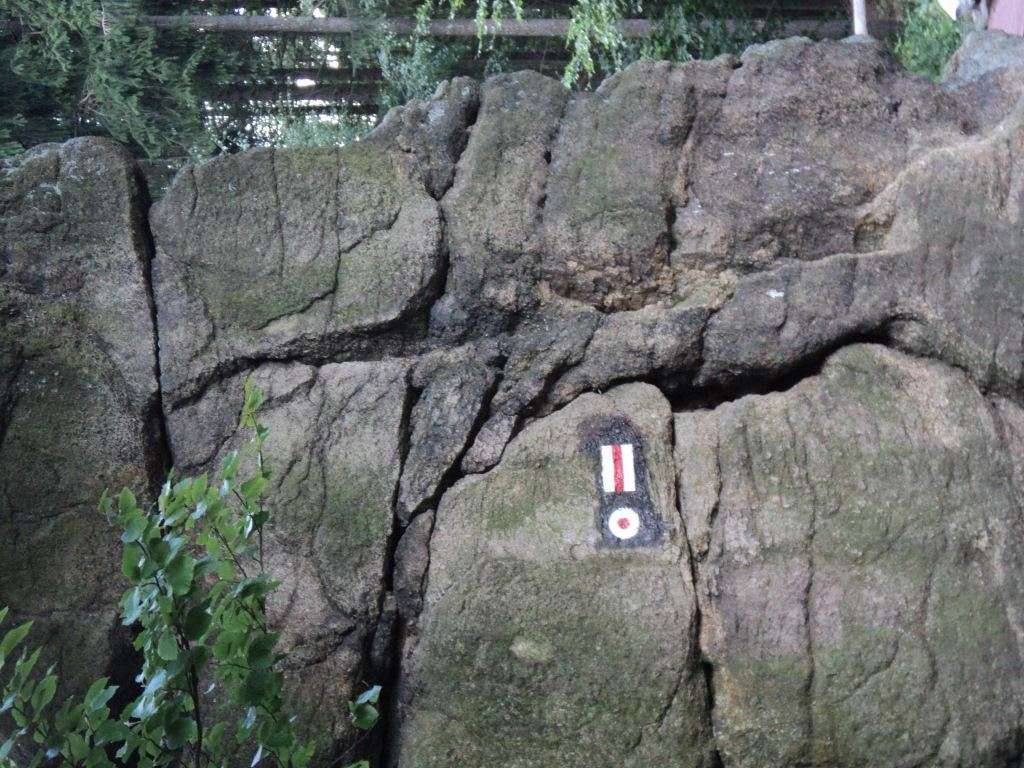
\includegraphics[width=5cm]{pict/slowik/v2/img1.jpg}
}
\subfigure[V2 2]{
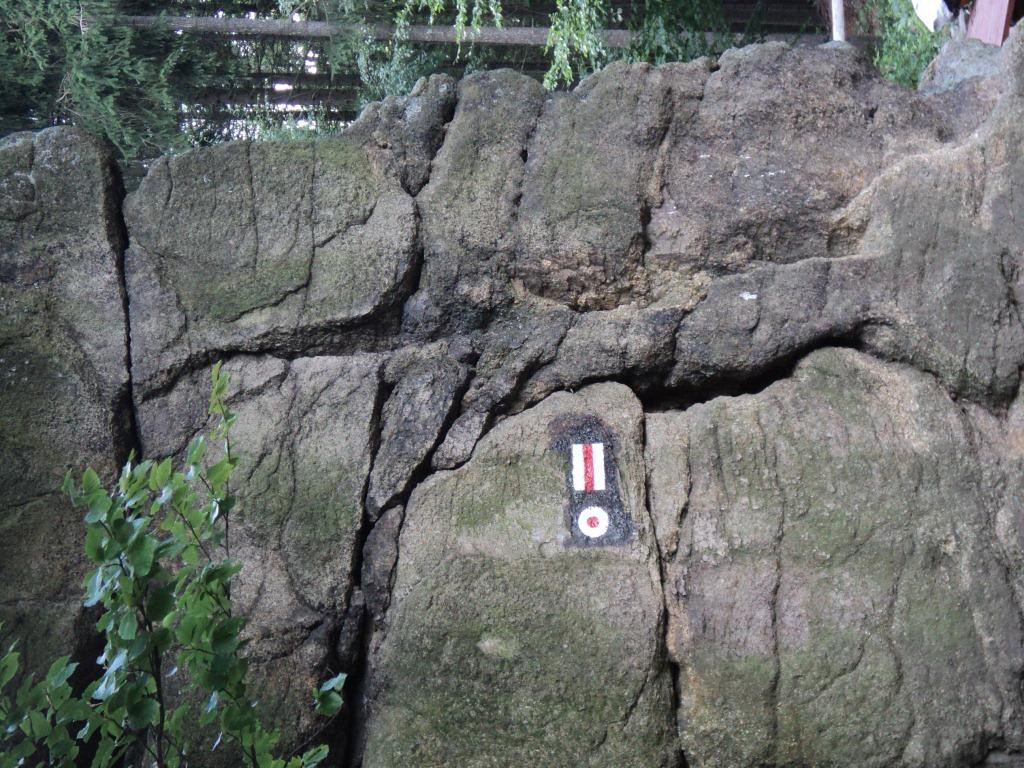
\includegraphics[width=5cm]{pict/slowik/v2/img2.jpg}
}
\subfigure[V2 3]{
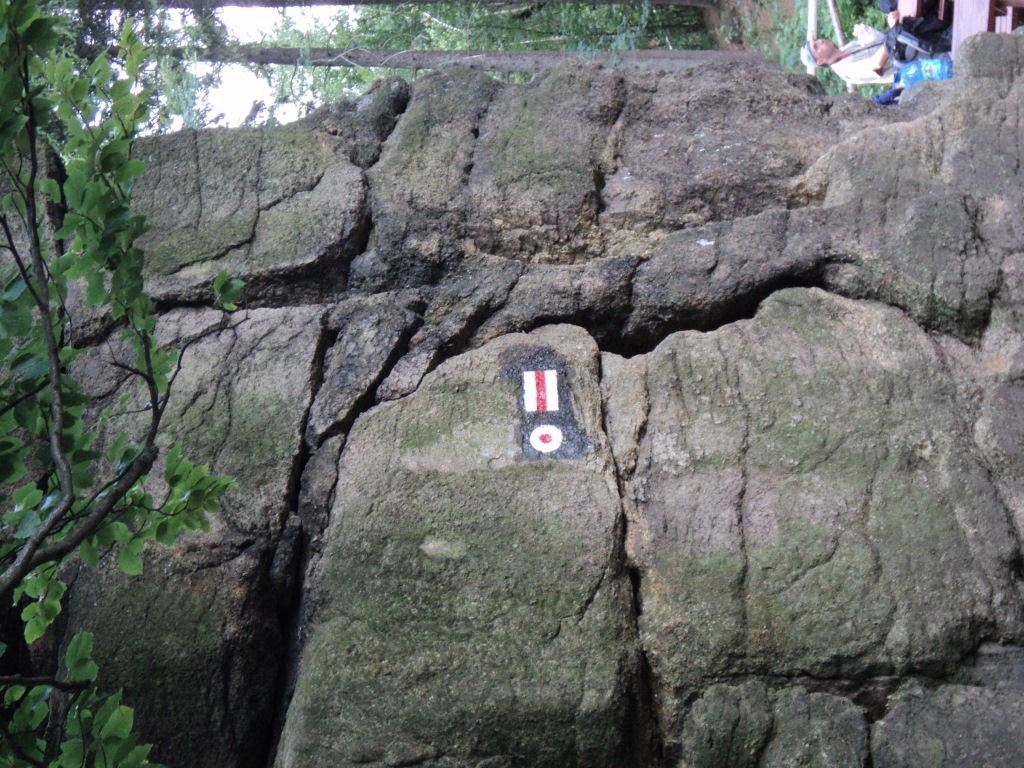
\includegraphics[width=5cm]{pict/slowik/v2/img3.jpg}
}
\subfigure[V2 4]{
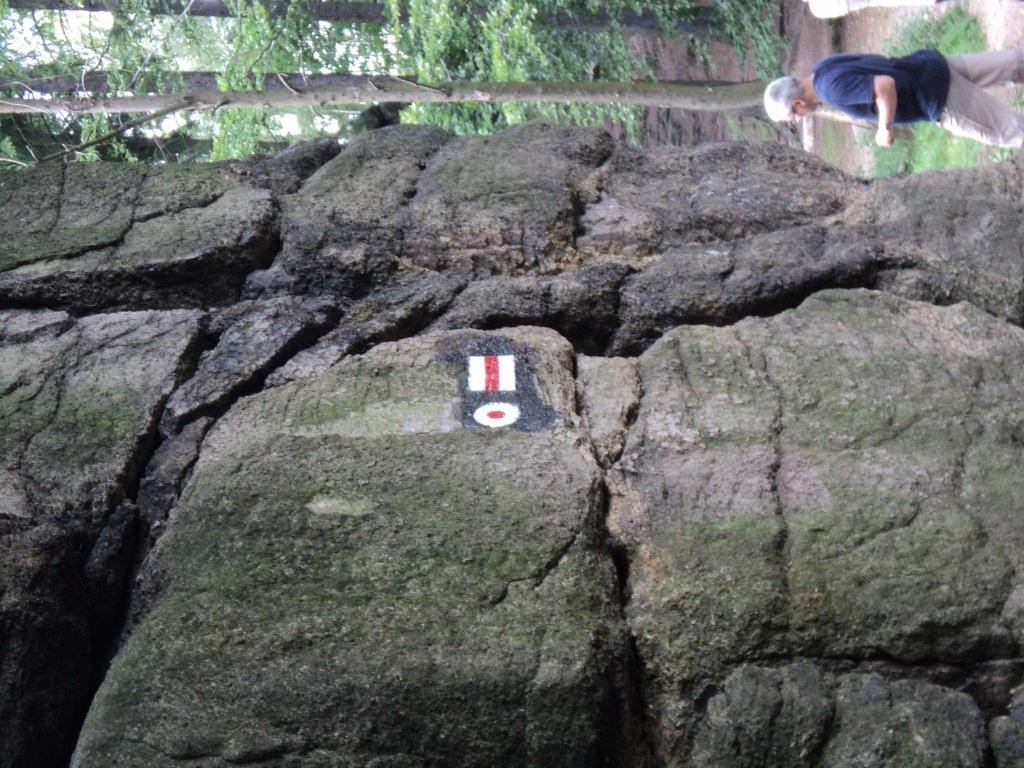
\includegraphics[width=5cm]{pict/slowik/v2/img4.jpg}
}
\subfigure[V2 5]{
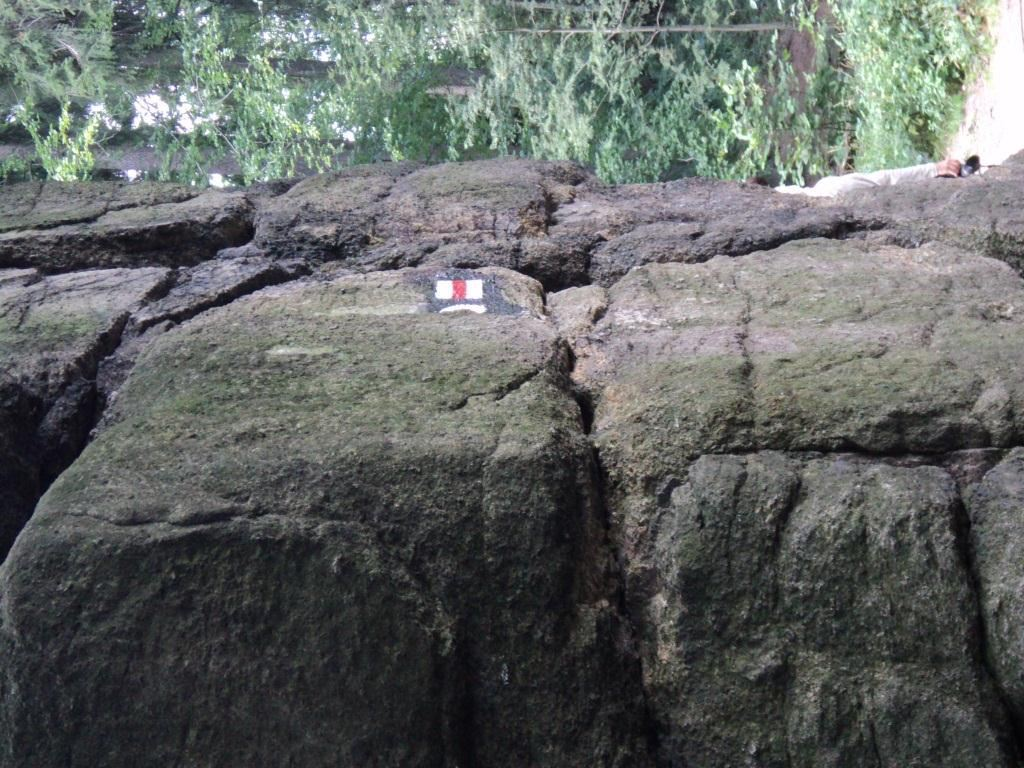
\includegraphics[width=5cm]{pict/slowik/v2/img5.jpg}
}
\subfigure[V2 6]{
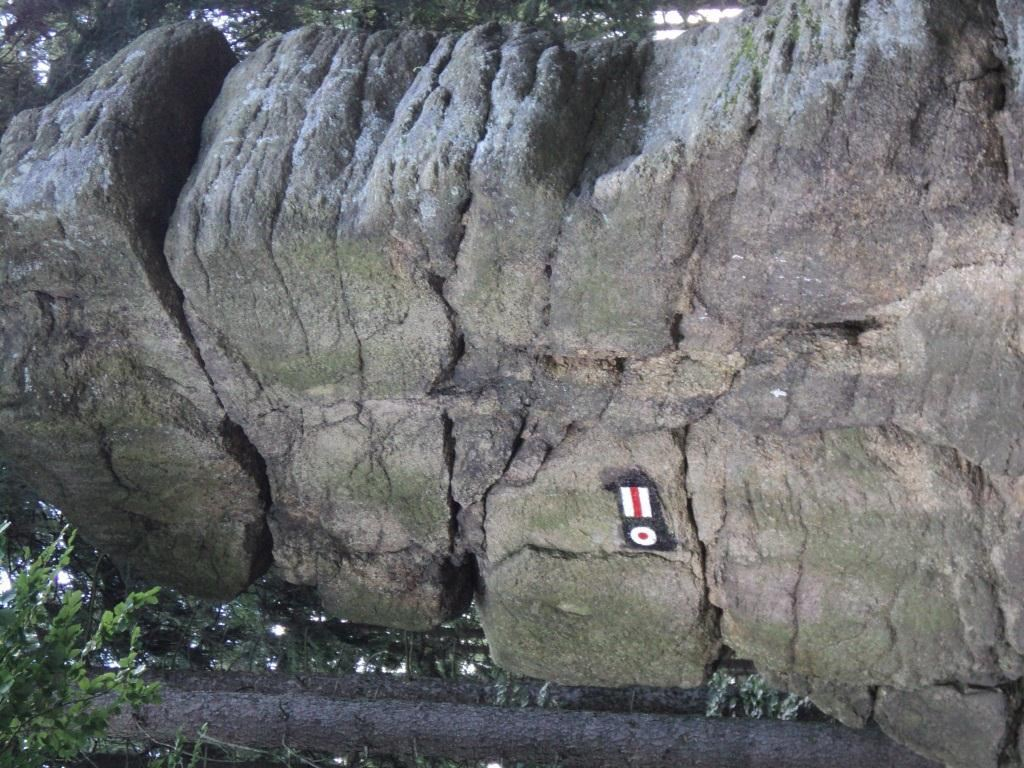
\includegraphics[width=5cm]{pict/slowik/v2/img6.jpg}
}
\caption{V2 - zbiór obrazów testowych}
\label{fig:v2_set}
\end{center}
\end{figure}



% Table generated by Excel2LaTeX from sheet 'm.v2 F'
\begin{table}[htbp]
  \centering
  \caption{V2 - ilość wyszukanych cech}
    \begin{tabular}{|c|r|r|r|r|r|}\hline
    
    obraz & \textbf{ORB} & \textbf{SIFT} & \textbf{SURF} & \textbf{STAR} & \textbf{FAST} \\\hline
    
   
    1 & 500 & 2389 & 11418 & 886 & 29038 \\
    2 & 500 & 2207 & 12586 & 1004 & 35894 \\
    3 & 500 & 2426 & 11923 & 873 & 31295 \\
    4 & 500 & 2568 & 10984 & 990 & 28111 \\
    5 & 500 & 2380 & 11698 & 1245 & 28736 \\
    6 & 500 & 2067 & 11915 & 551 & 27275 \\\hline
    \textbf{średnia} & \textbf{500} & \textbf{2340} & \textbf{11754} & \textbf{925} & \textbf{30058} \\
    \hline
    \end{tabular}%
  \label{tab:v2_f1}%
\end{table}%


\begin{figure}
\centering
\includegraphics[width=0.8\textwidth]{pict/slowik/v2/f1.png}
\caption{V2 - ilość wyszukanych cech}
\label{fig:v2_f1}
\end{figure}


% Table generated by Excel2LaTeX from sheet 'm.v2 F'
\begin{table}[htbp]
  \centering
  \caption{V2 - czas lokalizowania pojedynczego punktu charakterystycznego}
    \begin{tabular}{|c|c|c|c|c|c|}
    \hline
    obraz & \textbf{ORB} & \textbf{SIFT} & \textbf{SURF} & \textbf{STAR} & \textbf{FAST} \\
    \hline
    -  & [ms] & [ms] & [ms] & [ms] & [ms] \\
    1 & 0,134 & 0,098 & 0,170 & 0,097 & 0,001 \\
    2 & 0,154 & 0,104 & 0,166 & 0,087 & 0,001 \\
    3 & 0,144 & 0,096 & 0,168 & 0,100 & 0,001 \\
    4 & 0,142 & 0,094 & 0,172 & 0,088 & 0,001 \\
    5 & 0,146 & 0,100 & 0,169 & 0,071 & 0,001 \\
    6 & 0,126 & 0,111 & 0,169 & 0,158 & 0,001 \\\hline
    \textbf{średnia} & \textbf{0,141} & \textbf{0,100} & \textbf{0,169} & \textbf{0,100} & \textbf{0,001} \\
    \hline
    \end{tabular}%
  \label{tab:v2_f2}%
\end{table}%


\begin{figure}
\centering
\includegraphics[width=0.8\textwidth]{pict/slowik/v2/f2.png}
\caption{V2 - czas lokalizowania pojedynczego punktu charakterystycznego}
\label{fig:v2_f2}
\end{figure}

% Table generated by Excel2LaTeX from sheet 'm.v2 F'
\begin{table}[htbp]
  \centering
  \caption{V2 - czas generowania pojedynczego deskryptora punktu charakterystycznego}
    \begin{tabular}{|c|c|c|c|c|c|c|c|}\hline

    obraz & \textbf{ORB} & \textbf{SIFT} & \textbf{SURF} & \textbf{ST-BRIEF} & \textbf{ST-ORB} & \textbf{ST-SIFT} & \textbf{ST-SURF} \\\hline

    - & [ms] & [ms] & [ms] & [ms] & [ms] & [ms] & [ms] \\\hline
    1 & 0,102 & 0,234 & 0,210 & 0,019 & 0,017 & 1,073 & 0,098 \\
    2 & 0,100 & 0,242 & 0,206 & 0,018 & 0,016 & 1,036 & 0,098 \\
    3 & 0,100 & 0,235 & 0,209 & 0,019 & 0,017 & 1,094 & 0,100 \\
    4 & 0,102 & 0,229 & 0,212 & 0,018 & 0,016 & 1,088 & 0,099 \\
    5 & 0,102 & 0,232 & 0,216 & 0,017 & 0,014 & 0,882 & 0,095 \\
    6 & 0,102 & 0,243 & 0,205 & 0,022 & 0,022 & 0,902 & 0,096 \\\hline
    \textbf{średnia} & \textbf{0,101} & \textbf{0,236} & \textbf{0,210} & \textbf{0,019} & \textbf{0,017} & \textbf{1,012} & \textbf{0,098} \\\hline
    
    \end{tabular}%
  \label{tab:v2_f3}%
\end{table}%


\begin{figure}
\centering
\includegraphics[width=0.8\textwidth]{pict/slowik/v2/f3.png}
\caption{V2 - czas generowania pojedynczego deskryptora punktu charakterystycznego}
\label{fig:v2_f3}
\end{figure}


% Table generated by Excel2LaTeX from sheet 'm.v2 M'
\begin{table}[htbp]
  \centering
  \caption{V2 - powtarzalność wykrywanych cech}
    \begin{tabular}{|c|c|c|c|c|c|c|c|}\hline

    obrazy & \textbf{ORB} & \textbf{SIFT} & \textbf{SURF} & \textbf{ST-BRIEF} & \textbf{ST-ORB} & \textbf{ST-SIFT} & \textbf{ST-SURF} \\\hline

    -  & [\%] & [\%] & [\%] & [\%] & [\%] & [\%] & [\%] \\\hline
    1|2 & 22 & 38 & 44 & 67 & 64 & 69 & 27 \\
    1|3 & 4 & 20 & 12 & 30 & 25 & 33 & 4 \\
    1|4 & 1 & 1 & 0 & 3 & 2 & 3 & 2 \\
    1|5 & 0 & 0 & 0 & 2 & 2 & 1 & 1 \\
    1|6 & 2 & 2 & 1 & 3 & 3 & 6 & 1 \\\hline
    \textbf{średnia} & \textbf{6} & \textbf{12} & \textbf{11} & \textbf{21} & \textbf{19} & \textbf{22} & \textbf{7} \\\hline
    

    \end{tabular}%
  \label{tab:v2_m1}%
\end{table}%


\begin{figure}
\centering
\includegraphics[width=0.8\textwidth]{pict/slowik/v2/m1.png}
\caption{V2 - powtarzalność wykrywanych cech}
\label{fig:v2_m1}
\end{figure}

% Table generated by Excel2LaTeX from sheet 'm.v2 M'
\begin{table}[htbp]
  \centering
  \caption{V2 - procent poprawnych dopasowań}
    \begin{tabular}{|c|c|c|c|c|c|c|c|}\hline
    obrazy & \textbf{ORB} & \textbf{SIFT} & \textbf{SURF} & \textbf{ST-BRIEF} & \textbf{ST-ORB} & \textbf{ST-SIFT} & \textbf{ST-SURF} \\\hline
     - & [\%] & [\%] & [\%] & [\%] & [\%] & [\%] & [\%] \\\hline
    1|2 & 45 & 52 & 86 & 69 & 65 & 71 & 78 \\
    1|3 & 54 & 33 & 30 & 28 & 32 & 27 & 21 \\
    1|4 & 0 & 15 & 4 & 10 & 17 & 29 & 9 \\
    1|5 & 0 & 19 & 5 & 16 & 19 & 57 & 12 \\
    1|6 & 40 & 16 & 7 & 13 & 14 & 29 & 11 \\\hline
    \textbf{średnia} & \textbf{28} & \textbf{27} & \textbf{26} & \textbf{27} & \textbf{29} & \textbf{43} & \textbf{26} \\\hline
    
    \end{tabular}%
  \label{tab:v2_m2}%
\end{table}%


\begin{figure}
\centering
\includegraphics[width=0.8\textwidth]{pict/slowik/v2/m2.png}
\caption{V2 - procent poprawnych dopasowań}
\label{fig:v2_m2}
\end{figure}



\subsection{Dyskusja wyników}
Problem zmiany położenia obserwatora wydaje się być najtrudniejszym dla badanych algorytmów. O ile charakterystyki czasowe i ilościowe dla obrazów w ramach pojedynczego zbioru pozostają stałe, o tyle w przypadku wskaźników dopasowań obserwujemy duże zróżnicowanie wyników i lawinowy spadek skuteczności wraz ze zmiana położenia. Klasyfikacja w dziedzinach ilości punktu, czasów detekcji i opisywanie nie różni się w zasadniczy sposób od tych zaobserwowanych w poprzednich badaniach.

W trakcie konstruowania zbioru testowego obserwator przemieszczał się średnio o 2 metry pomiędzy kolejnymi ujęciami. Badania wykazują dużą wrażliwość algorytmów na przemieszczenie obserwatora powyżej 4 metrów. Powtarzalność dla takiej transformacji w najlepszych warunkach wynosi około 30\%, by finalnie spaść niemal do 0. Zjawisko to jest obserwowane dla obu zestawów.

Procent dobrze dopasowanych punktów jest wskaźnikiem silnie powiązanym z powtarzalnością. W sytuacji gdy powtarzalność spada do 0, bezzasadnym staje się dyskusja poprawności. Biorąc pod uwagę te pary obrazów z niezerową powtarzalnością, najlepsze wyniki w zależności od sceny osiągają algorytmy ORB i STAR-SIFT.

\FloatBarrier
\newpage
\section{Zmiana skali}
\subsection{Z1}
Transformacja: Zmiana skali\\
Rejon: Krzywa Turnia\\
Powiększenie: Duże\\
Oświetlenie: Umiarkowane/Mieszane\\
Rozdzielczość: $1024 \times 768$

\begin{figure}[!htb]
\begin{center}
\subfigure[z1 1]{
\includegraphics[width=5cm]{pict/slowik/z1/img1.jpg}
}
\subfigure[z1 2]{
\includegraphics[width=5cm]{pict/slowik/z1/img2.jpg}
}
\subfigure[z1 3]{
\includegraphics[width=5cm]{pict/slowik/z1/img3.jpg}
}
\subfigure[z1 4]{
\includegraphics[width=5cm]{pict/slowik/z1/img4.jpg}
}
\subfigure[z1 5]{
\includegraphics[width=5cm]{pict/slowik/z1/img5.jpg}
}
\subfigure[z1 6]{
\includegraphics[width=5cm]{pict/slowik/z1/img6.jpg}
}
\caption{Z1 - zbiór obrazów testowych}
\label{fig:z1_set}
\end{center}
\end{figure}



% Table generated by Excel2LaTeX from sheet 'm.z1 F'
\begin{table}[htbp]
  \centering
  \caption{Z1 - ilość wyszukanych cech}
    \begin{tabular}{|c|r|r|r|r|r|}\hline
    
    obraz & \textbf{ORB} & \textbf{SIFT} & \textbf{SURF} & \textbf{STAR} & \textbf{FAST} \\\hline
    
   
    1 & 500 & 2318 & 10357 & 874 & 24877 \\
    2 & 500 & 2360 & 10257 & 833 & 24590 \\
    3 & 500 & 2303 & 9109 & 763 & 17416 \\
    4 & 500 & 2281 & 10120 & 1033 & 24754 \\
    5 & 500 & 2503 & 9943 & 1220 & 23616 \\
    6 & 500 & 3012 & 9473 & 1485 & 21403 \\\hline
    \textbf{średnia} & \textbf{500} & \textbf{2463} & \textbf{9877} & \textbf{1035} & \textbf{22776} \\
    \hline
    \end{tabular}%
  \label{tab:z1_f1}%
\end{table}%


\begin{figure}
\centering
\includegraphics[width=0.8\textwidth]{pict/slowik/z1/f1.png}
\caption{Z1 - ilość wyszukanych cech}
\label{fig:z1_f1}
\end{figure}


% Table generated by Excel2LaTeX from sheet 'm.z1 F'
\begin{table}[htbp]
  \centering
  \caption{Z1 - czas lokalizowania pojedynczego punktu charakterystycznego}
    \begin{tabular}{|c|c|c|c|c|c|}
    \hline
    obraz & \textbf{ORB} & \textbf{SIFT} & \textbf{SURF} & \textbf{STAR} & \textbf{FAST} \\
    \hline
    -  & [ms] & [ms] & [ms] & [ms] & [ms] \\\hline
    1 & 0,132 & 0,099 & 0,176 & 0,100 & 0,001 \\
    2 & 0,132 & 0,098 & 0,174 & 0,104 & 0,001 \\
    3 & 0,120 & 0,103 & 0,180 & 0,114 & 0,001 \\
    4 & 0,144 & 0,102 & 0,175 & 0,086 & 0,001 \\
    5 & 0,142 & 0,096 & 0,177 & 0,072 & 0,001 \\
    6 & 0,146 & 0,083 & 0,178 & 0,060 & 0,001 \\\hline
    \textbf{średnia} & \textbf{0,136} & \textbf{0,097} & \textbf{0,177} & \textbf{0,089} & \textbf{0,001} \\
    \hline
    

    \end{tabular}%
  \label{tab:z1_f2}%
\end{table}%


\begin{figure}
\centering
\includegraphics[width=0.8\textwidth]{pict/slowik/z1/f2.png}
\caption{Z1 - czas lokalizowania pojedynczego punktu charakterystycznego}
\label{fig:z1_f2}
\end{figure}

% Table generated by Excel2LaTeX from sheet 'm.z1 F'
\begin{table}[htbp]
  \centering
  \caption{Z1 - czas generowania pojedynczego deskryptora punktu charakterystycznego}
    \begin{tabular}{|c|c|c|c|c|c|c|c|}\hline

    obraz & \textbf{ORB} & \textbf{SIFT} & \textbf{SURF} & \textbf{ST-BRIEF} & \textbf{ST-ORB} & \textbf{ST-SIFT} & \textbf{ST-SURF} \\\hline

    - & [ms] & [ms] & [ms] & [ms] & [ms] & [ms] & [ms] \\\hline
    1 & 0,100 & 0,234 & 0,194 & 0,019 & 0,017 & 1,292 & 0,104 \\
    2 & 0,100 & 0,231 & 0,195 & 0,019 & 0,018 & 1,414 & 0,106 \\
    3 & 0,104 & 0,237 & 0,197 & 0,020 & 0,018 & 1,507 & 0,107 \\
    4 & 0,102 & 0,243 & 0,195 & 0,018 & 0,015 & 1,370 & 0,105 \\
    5 & 0,104 & 0,235 & 0,198 & 0,017 & 0,015 & 1,245 & 0,102 \\
    6 & 0,100 & 0,222 & 0,201 & 0,016 & 0,014 & 1,213 & 0,100 \\\hline
    \textbf{średnia} & \textbf{0,102} & \textbf{0,234} & \textbf{0,197} & \textbf{0,018} & \textbf{0,016} & \textbf{1,340} & \textbf{0,104} \\\hline
    
   
   

    \end{tabular}%
  \label{tab:z1_f3}%
\end{table}%


\begin{figure}
\centering
\includegraphics[width=0.8\textwidth]{pict/slowik/z1/f3.png}
\caption{Z1 - czas generowania pojedynczego deskryptora punktu charakterystycznego}
\label{fig:z1_f3}
\end{figure}


% Table generated by Excel2LaTeX from sheet 'm.z1 M'
\begin{table}[htbp]
  \centering
  \caption{Z1 - powtarzalność wykrywanych cech}
    \begin{tabular}{|c|c|c|c|c|c|c|c|}\hline

    obrazy & \textbf{ORB} & \textbf{SIFT} & \textbf{SURF} & \textbf{ST-BRIEF} & \textbf{ST-ORB} & \textbf{ST-SIFT} & \textbf{ST-SURF} \\\hline

    -  & [\%] & [\%] & [\%] & [\%] & [\%] & [\%] & [\%] \\\hline
    1|2 & 37 & 38 & 33 & 46 & 37 & 63 & 12 \\
    1|3 & 11 & 16 & 12 & 7 & 4 & 27 & 5 \\
    1|4 & 5 & 9 & 8 & 4 & 3 & 18 & 3 \\
    1|5 & 3 & 7 & 5 & 3 & 2 & 7 & 2 \\
    1|6 & 1 & 4 & 2 & 1 & 1 & 1 & 1 \\\hline
    \textbf{średnia} & \textbf{12} & \textbf{15} & \textbf{12} & \textbf{12} & \textbf{10} & \textbf{23} & \textbf{4} \\\hline
    
    

    \end{tabular}%
  \label{tab:z1_m1}%
\end{table}%


\begin{figure}
\centering
\includegraphics[width=0.8\textwidth]{pict/slowik/z1/m1.png}
\caption{Z1 - powtarzalność wykrywanych cech}
\label{fig:z1_m1}
\end{figure}

% Table generated by Excel2LaTeX from sheet 'm.z1 M'
\begin{table}[htbp]
  \centering
  \caption{Z1 - procent poprawnych dopasowań}
    \begin{tabular}{|c|c|c|c|c|c|c|c|}\hline
    obrazy & \textbf{ORB} & \textbf{SIFT} & \textbf{SURF} & \textbf{ST-BRIEF} & \textbf{ST-ORB} & \textbf{ST-SIFT} & \textbf{ST-SURF} \\\hline
     - & [\%] & [\%] & [\%] & [\%] & [\%] & [\%] & [\%] \\\hline
    1|2 & 69 & 69 & 71 & 54 & 67 & 66 & 42 \\
    1|3 & 47 & 51 & 42 & 26 & 9 & 59 & 22 \\
    1|4 & 32 & 47 & 41 & 12 & 10 & 47 & 21 \\
    1|5 & 24 & 49 & 36 & 15 & 13 & 45 & 26 \\
    1|6 & 19 & 38 & 19 & 12 & 13 & 52 & 16 \\\hline
    \textbf{średnia} & \textbf{38} & \textbf{51} & \textbf{42} & \textbf{24} & \textbf{22} & \textbf{54} & \textbf{25} \\\hline
    
    \end{tabular}%
  \label{tab:z1_m2}%
\end{table}%


\begin{figure}
\centering
\includegraphics[width=0.8\textwidth]{pict/slowik/z1/m2.png}
\caption{Z1 - procent poprawnych dopasowań}
\label{fig:z1_m2}
\end{figure}

\FloatBarrier
\subsection{Dyskusja wyników}
Większość algorytmów niezależnie od stopnia przybliżenia generuje zbliżoną liczbę punktów charakterystycznych. Podobnie jak w poprzednich testach najwięcej cech lokalizuje algorytm FAST, potem SURF, następnie SIFT, STAR i stało wartościowy ORB.

Charakterstyki czasowe również pozostają stałe dla obrazów w zbiorze. Najwolniej punkty lokalizują algorytmy SURF i ORB, z kolei najwolniejszym deskryptorem jest kooeprujący z algorytmem STAR, deskryptor SIFT.

Metoda ta jednak osiąga najlepszy współczynnik powtarzalności. Dla większości algorytmów wskaźnik ten znacząco spada przy zmianie skali większej niż $0,5$.

Metoda STAR-SIFT osiąga również najlepsze wyniki pod względem trafności dopasowań. Nieznacznie gorzej przy niej wypada czysty algorytm SIFT. Pozostałe metody w tym obszarze rzadko osiągają poprawność przekraczającą $30\% $ .
